\documentclass[]{foi} % zakomentirati za pisanje rada na engleskom jeziku
% \documentclass[english]{foi} % odkomentirati za pisanje rada na engleskom jeziku
\usepackage[utf8]{inputenc}
\usepackage{lipsum}
\usepackage{float}

\vrstaRada{\zavrsni}
% \zavrsni ili \diplomski ili \seminar ili \projekt

\title{Računalni vid i prepoznavanje objekata pomoću biblioteke OpenCV}
\predmet{}
% ostaviti prazno ako \vrstaRada nije \projekt ili \seminar
% \predmetBP ili \predmetDP ili \predmetTBP ili \predmetVAS

\author{Petar Matišić} % ime i prezime studenta/studentice
\spolStudenta{\musko} % \zensko ili \musko

\mentor{Bogdan Okreša Đurić} % ime i prezime mentora
\spolMentora{\musko} % \zensko ili \musko
\titulaProfesora{dr. sc.}
% HR: dr. sc.  / doc. dr. sc. / izv. prof. dr. sc. / prof. dr. sc. 
% EN: -prazno- / Asst. Prof.  / Assoc. Prof.       / Full Prof.

\godina{2022}
\mjesec{rujan} % mjesec obrane rada ili projekta

\indeks{0016145882} % broj indeksa ili JMBAG

\smjer{Informacijski sustavi}
% (ili:
%     Informacijski sustavi, 
%     Poslovni sustavi, 
%     Ekonomika poduzetništva, 
%     Primjena informacijske tehnologije u poslovanju, 
%     Informacijsko i programsko inženjerstvo, 
%     Baze podataka i baze znanja, 
%     Organizacija poslovnih sustava, 
%     Informatika u obrazovanju
% )


\sazetak{U ovome radu obrađuje se problematika računalnog vida, odnosno područje koje je posljednjih godina uspjelo napraviti veliki skok i uspjelo nadmašiti ljude u nekim zadacima povezanima s otkrivanjem i označavanjem objekata. Predstavljena je povijest problema te njegov opis. Zatim su predstavljeni neki od načina rješavanja ovoga problema. Osim obrade navedenog, također, cilj izučavanja u ovom radu je i njena teorijska podloga koja seže iz dubokog učenja i neuronskih mreža koje danas predstavljaju temelj za izradu raznolikih modela vezanih za strojno učenje i njegove aplikacije. Nabrojana su područja primjene računalnog vida, te je prikazan rad kroz primjere zasnovan za konceptima navedenih područja. Vezano za primjere, na kraju su napravljene dvije različite implementacije, od kojih jedna prepoznaje gestikulacije ruke, a druga gdje se također pomoću ruke može prikazati upravljanje i manipulacija pokazivačem na zaslonu.}

\kljucneRijeci{računalni vid; duboko učenje; neuronska mreža; python; ruka; opencv}



\begin{document}

\maketitle

\tableofcontents

\makeatletter \def\@dotsep{4.5} \makeatother
\pagestyle{plain}



\chapter{Uvod}

Kraj 20. stoljeća započeo je sve bržim razvojem elektronike, računala i softvera koji je omogućio bolja računala. Danas se nove tehnologije i softver razvijaju tako brzo da se inovacije pojavljuju gotovo svaki dan u \textit{IT} svijetu. "Obični" programeri više ne mogu pratiti sve trendove i pravce razvoja programskih jezika, već fokus rada prelazi na jedno područje. Jedno od takvih područja, koje je novo, ali se rapidno razvija, je računalni vid.

Računalni vid daje računalima sposobnost "vidjeti", odnosno razumjeti što je na fotografiji ili videu. Računalni vid nam omogućuje razvoj potpuno novih aplikacija za svakodnevnu upotrebu. Njegova glavna svrha može biti npr. sigurnost i zaštita, kao što su: zaštita ljudi, zaštita podataka, sprječavanje smrti, otkriće raka itd.

Uz pomoć računalnog vida, troškovi se mogu smanjiti u usporedbi s troškovima obavljanja istih poslova pri korištenju ljudskih usluga, uz relativno nisku ekonomsku potrošnju. Daljnjim razvojem računalnog vida može se smanjiti broj pogrešaka u analizi određenih informacija u odnosu na ljudski faktor. U svakodnevnom životu, računalni vid može pomoći u rješavanju kriminalnih radnji, detektirao bi osobe koje su počinile neku vrstu nedjela ili kaznenog djela. Ljudska svijest o postojanju nekakvog sustava nadzora smanjuje učestalost kriminalnih aktivnosti. Isto tako, njegova pojava može spriječiti mnoge prometne nesreće, pomoći i razviti medicinske usluge, poput otkrivanja bolesti kod ljudi, otkrivanja tumora itd. Računalni vid svakim danom ima nove zahtjeve koje treba implementirati u svakodnevne aktivnosti, a jedan od njih je prepoznavanje kupaca i njihovih dosadašnjih kupovnih navika i potreba. Danas, dakle, postoje  automobili koji se upravljaju na vlastiti pogon, mobiteli koji se mogu otključati samo uz pomoć algoritama za prepoznavanje lica i mnoge druge inovacije u svakodnevnom životu, zahvaljujući pojedincima koji su prepoznali mogućnosti koje nudi računalni vid. Još uvijek nismo svjesni činjenice koliko je ovaj segment snažan i primjenjiv za razvoj te kolika će biti njegova korisnost za buduće sinergije u suradnji računala/stroja i ljudi (npr. zajednički rad u proizvodnji, vožnji i sl.).

Rad bi trebao objasniti kako računalo može prepoznati postoji li određena vrsta objekta na slici, poput prometnog znaka, ljudskog lica, tumora na medicinskoj slici i još mnogo toga.
Računala mogu koristiti širi raspon valnih duljina svjetlosti za računalni vid za razliku od ljudskog oka. Znanje računalnog vida primjenjivo je u svim znanstvenim disciplinama računarstva i mnogo drugih znanosti.

\chapter{Duboko učenje}

\hspace{20 mm}

\begin{figure}[!ht]
    \centering
    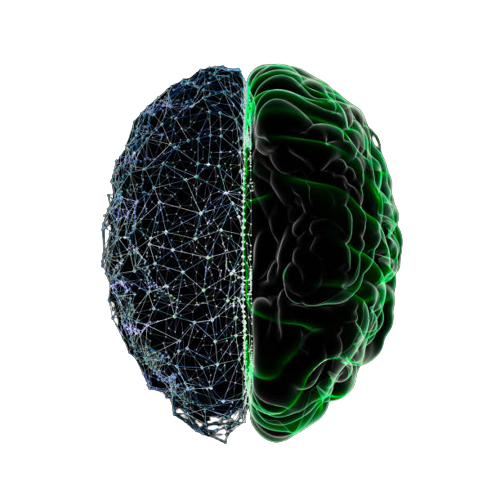
\includegraphics[width=1\textwidth]{slike/mozak.png}
    \caption{Neuronska mreža i polutka mozga; prema: \cite{deep}}
    \label{fig:struce}
\end{figure}

\hspace{20 mm}

\begin{center}
\textit{“Predviđanje budućnosti nije magija, to je umjetna inteligencija.”} -- Dave Waters \cite{deep}.    
\end{center}

\newpage
\section{Definiranje pojmova}

Tijekom proteklih nekoliko godina duboko učenje postalo je popularan pojam u svijetu tehnologije. Prije nego što se detaljnije objasni duboko učenje, njegovi algoritmi i primjene, prva stvar koja je najbitnija u razumijevanju dubokog učenja je što je to stvarno duboko učenje.

Duboko učenje \cite{builtin1} je potpodručje strojnog učenja koje se bavi algoritmima inspiriranim strukturom i funkcijom mozga. Duboko učenje je automatski i podskup umjetne inteligencije jer samim time strojno učenje spada pod područje umjetne inteligencije.

\vspace{10mm}
\begin{figure}[!ht]
    \centering
    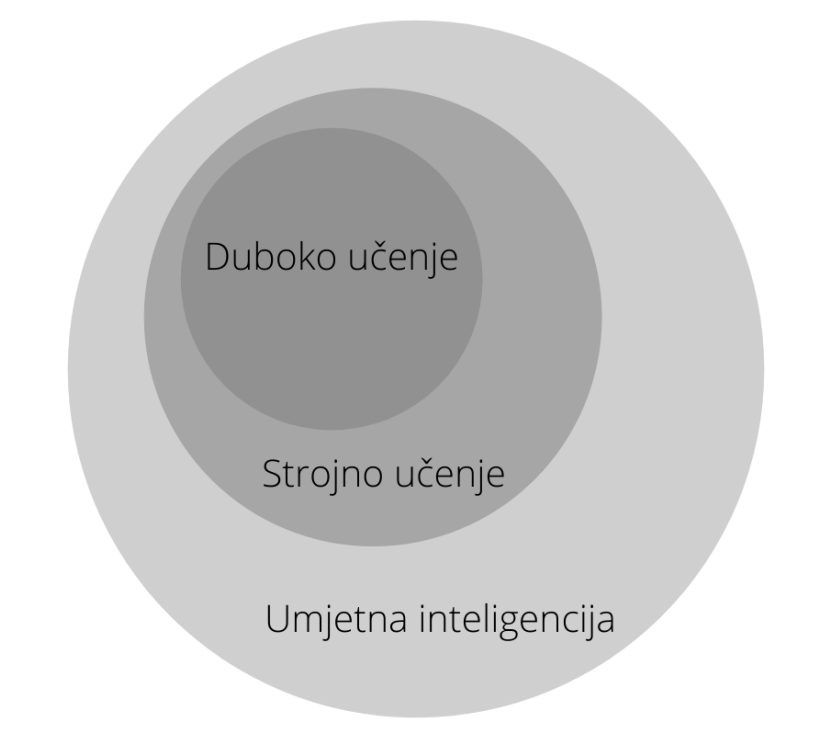
\includegraphics[width=0.8\textwidth]{slike/podjela.png}
    \caption{Potpodručja umjetne inteligencije; prema: \cite{builtin1}}
    \label{fig:podjela}
\end{figure}
\vspace{10mm}

Glavni cilj \cite{builtin1} umjetne inteligencije je osigurati skup algoritama i tehnika koje se mogu koristiti za rješavanje problema koji su intuitivni i samoizvršivi za ljude, ali predstavljaju veliki izazov za računala. Dobar primjer ove vrste problema je tumačenje i razumijevanje sadržaja slike, nešto što ljudi mogu učiniti bez napora, a što je strojevima vrlo teško, kao što je spomenuto u uvodu. Razlika između dubokog učenja, strojnog učenja i umjetne inteligencije je prikazana na slici \ref{fig:podjela}.

\newpage
Kada je riječ o pojmu dubokog učenja, obično se misli na neuronsku mrežu koja većinom sadrži velik broj slojeva \cite{builtin1}. Dakle, duboko učenje zapravo je vrlo širok pojam jer ne postoji univerzalno prihvaćen broj slojeva koje neuronska mreža mora imati da bi se klasificirala kao duboka neuronska mreža. Za razliku od tradicionalnog strojnog učenja koje uzima skup slika i primjenjuje ručno definirani algoritam izdvajanja značajki te, ili čak ručno izdvajanje značajki, provodi obuku klasifikatora koji se temelje na tim značajkama (Slika \ref{fig:mlvsdl}), duboko učenje temelji se na principu slaganja sloj-po-sloj, koje automatski uče složenije i apstraktnije značajke u usporedbi s tradicionalnim strojnim učenjem.

\vspace{10mm}
\begin{figure}[!ht]
    \centering
    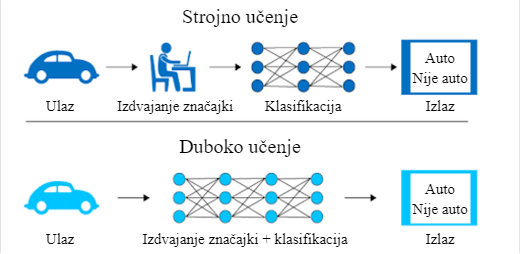
\includegraphics[width=1\textwidth]{slike/mlvsdl.png}
    \caption{Razlika dubokog i strojnog učenja; prema: \cite{builtin1}}
    \label{fig:mlvsdl}
\end{figure}
\vspace{10mm}

Za većinu problema, neki klasični algoritmi strojnog učenja proizvest će dovoljno dobre modele \cite{tds2}. Za druge, ozbiljnije probleme, klasični algoritmi strojnog učenja u prošlosti nisu imali dovoljno dobre rezultate. Jedno od područja gdje se duboko učenje često naglašava je obrada prirodnog jezika, uključujući prijevod jezika, automatsko sažimanje, analitiku, morfološku segmentaciju, analizu osjećaja i prepoznavanje govora \cite{tds1}.

Još jedno glavno područje dubokog učenja je klasifikacija slika \cite{tds1}, koja primarno uključuje detekciju objekta na slici, prepoznavanje lica i identiteta osobe, identificiranje objekata na slikama kao što su znakovi za zaustavljanje, pješaci i oznake traka. Nadalje, duboko učenje se uspješno koristi za predviđanje molekularnih interakcija kako bi farmaceutske tvrtke mogle dizajnirati nove lijekove.

\newpage
\section{Algoritmi}

Algoritmi dubokog i strojnog učenja \cite[str. 98-105]{deep} obično se dijele na nadzirane (podaci o obuci označeni su točnim odgovorima) i nenadzirane (odgovori se ne prikazuju tijekom obuke) (Slika \ref{fig:nvsnn}). Problemi algoritama nadziranog strojnog učenja dalje se dijele na klasifikaciju (predviđanje nenumeričkih odgovora) i regresiju (predviđanje numeričkih odgovora). Nenadzirano učenje dalje se dijeli na grupiranje (pronalaženje grupa sličnih predmeta), pridruživanje (pronalaženje zajedničkih nizova predmeta) i smanjenje dimenzionalnosti (projekcija, odabir značajki i ekstrakcija značajki).

Kada se govori o nadziranom učenju \cite{tds1}, takvo učenje se definira korištenjem označenih skupova podataka za obuku algoritama koji klasificiraju podatke ili točno predviđaju ishode. Kako se ulazni podaci unose u model, on prilagođava svoje vrijednosti sve dok se model pravilno ne prilagodi. Kao što je spomenuto, algoritmi nadziranog učenja mogu se podijeliti s obzirom na klasifikaciju i regresiju. Problem klasifikacije \cite{tds1} zahtijeva izbor između dvije ili više klasa, obično s vjerojatnošću za svaku klasu. Primjerice, najpoznatiji algoritmi \cite[str. 137]{deep} koji riješavaju probleme klasifikacija su stabla odlučivanja, k-najbližih susjeda i algoritam stroja potpornog vektora (eng. \textit{Support Vector Machine (SVM)}).
Neki primjeri \cite{tds2} klasifikacije su česti primjeri filtriranja neželjene pošte ili spam-a, otkrivanje jezika na određenim web stranicama ili dokumentima, dok primjeri regresije su predviđanje cijena dionica nekih tvrtki, analiza ponude i potražnje itd.

Problem regresije koji je također jedan od problema nadziranog učenja, traži od modela predviđanje numeričkih vrijednosti. Na primjer, linearna regresija \cite[str. 105, 106]{deep} koristi se za određivanje odnosa između zavisne varijable i jedne ili više nezavisnih varijabli, obično za predviđanje budućih ishoda. Kako se broj nezavisnih varijabli povećava, linearna regresija postaje višestruka. Uz linearnu, postoji i logistička regresija koja se odabire kada je zavisna varijabla kategorička, što znači da imaju binarne izlaze kao što su "točno" i "netočno" ili "da" i "ne".

\begin{figure}[!ht]
    \centering
    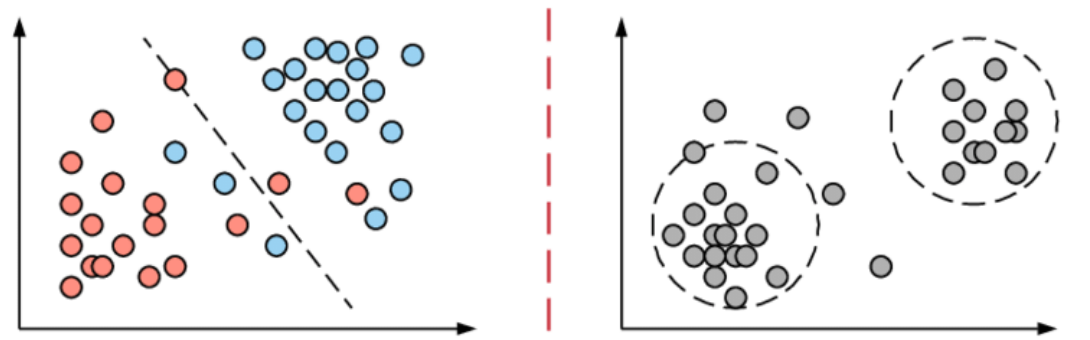
\includegraphics[width=1\textwidth]{slike/nvsnn.png}
    \caption{Nadzirano učenje (lijevo) i nenadzirano učenje (desno); prema: \cite{deep}}
    \label{fig:nvsnn}
\end{figure}

Za razliku od nadziranog, nenadzirano učenje \cite{tds1, deep} koristi neoznačene podatke. Iz tih podataka pronalazi uzorke koji pomažu u rješavanju problema klasteriranja ili povezivanja. Uobičajeni algoritmi klasteriranja su hijerarhijski, k-srednje vrijednosti i Gaussovi modeli \cite[str. 142]{deep}.

\newpage
\section{Neuronske mreže}

Sada kada je poznat pojam dubokog učenja, njegove primjene i važnosti, može se prijeći na pojam umjetne neuronske mreže i njenih operacija.

Da bi se razumjelo kako radi umjetni neuron, prvo se treba razumjeti kako radi biološki neuron.
Dakle, neuron ima tijelo, dendrite i akson \cite{tds1} (Slika \ref{fig:bnn}). Dendriti primaju informacije ili signale od drugih neurona koji se s njima povezuju. Obrada informacija odvija se u tijelu stanice odnosno ono preuzima sve informacije koje dolaze iz različitih dendrita i obrađuje te informacije. Aksoni šalju izlazni signal drugom neuronu za protok informacija.

\begin{figure}[!ht]
    \centering
    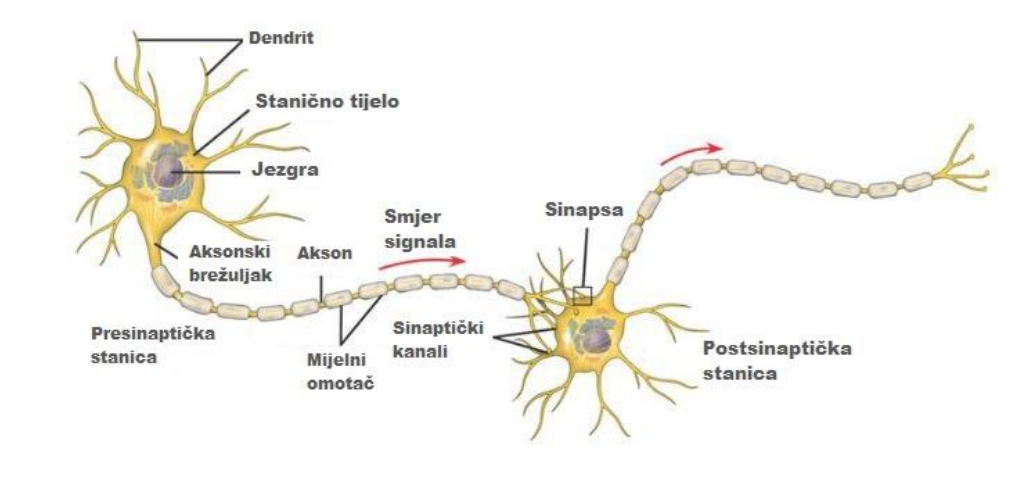
\includegraphics[width=1\textwidth]{slike/bnn.png}
    \caption{Biološka neuronska mreža; prema: \cite{builtin1}}
    \label{fig:bnn}
\end{figure}

\begin{figure}[!ht]
    \centering
    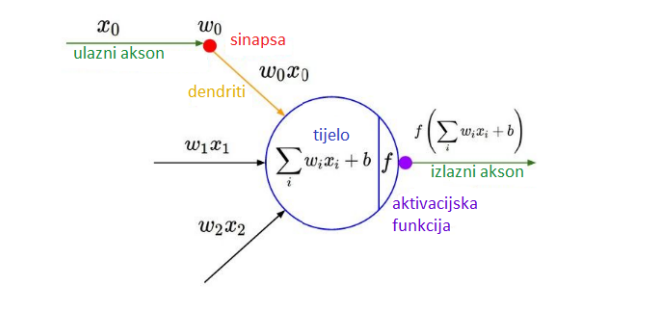
\includegraphics[width=1\textwidth]{slike/neuron.png}
    \caption{Umjetni neuron; prema: \cite{principles}}
    \label{fig:neuron}
\end{figure}


Gledajući u sliku \ref{fig:neuron}, može se primjetiti kako umjetni neuron replicira biološki neuron. Matematički, on se prikazuje kao \cite{principles}:

\[
y_k=\varphi\left(\sum_{i=1}^m x_i \cdot w_{k i}+b_k\right)
\]

gdje
\begin{itemize}
    \item $x_1, x_2, x_3, ..., x_m$ su ulazni signali,
    \item $w_1, w_2, w_3, ..., w_m$ su odgovarajuće težine neurona,
    \item $b_k$ je pomak koji može imati pozitivnu ili negativnu vrijednost te imati utjecaj na povećanje ili smanjenje vrijednosti ulaznih signala u aktivacijsku funkciju,
    \item $\varphi$ je aktivacijska funkcija koja prima ulazne signale od susjednih neurona te ih zatim zbraja i na taj zbroj djeluje nekom određenom transformacijom uzimajući u obzir vrijednost pomaka $b_k$.
\end{itemize}

Ulaz u neuron predstavlja ulazni sloj, sami neuron je u biti skriveni sloj, a izlaz do posljednjeg neurona je izlazni sloj \cite{builtin1}.

\begin{figure}[!ht]
    \centering
    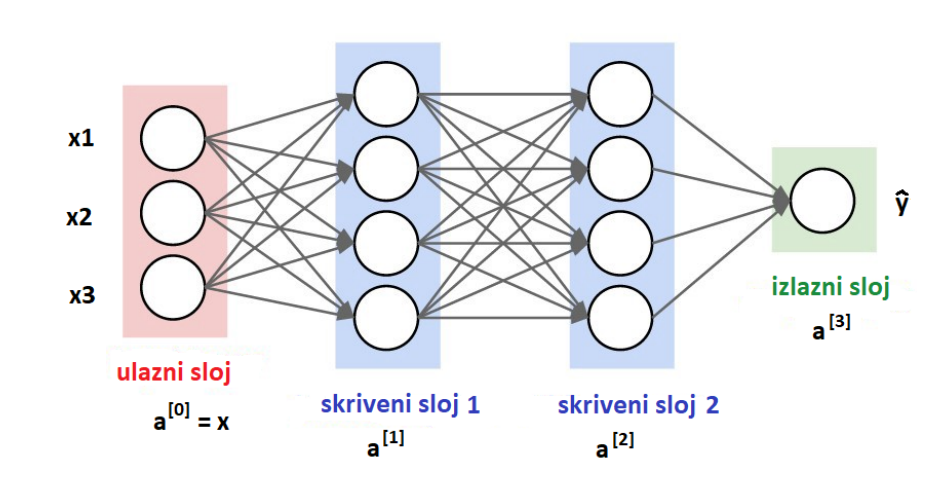
\includegraphics[width=1\textwidth]{slike/mreza.png}
    \caption{Arhitektura neuronske mreže; prema: \cite{builtin1}}
    \label{fig:arhitektura}
\end{figure}

Tipična arhitektura neuronske mreže prikazana je na slici \ref{fig:arhitektura} i sastoji se od nekoliko slojeva od kojih su već prije spomenuti najbitniji slojevi -- ulazni, skriveni i izlazni. Na sljedećim slikama istaknut je matematički proces učenja neuronske mreže \cite{builtin1}.

\begin{figure}[!ht]
    \centering
    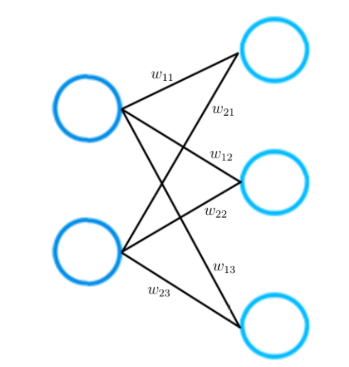
\includegraphics[width=0.4\textwidth]{slike/struktura.png}
    \caption{Veze slojeva; prema: \cite{builtin1}}
    \label{fig:struktura}
\end{figure}

Veza između dva neurona predstavljena je s vrijednošću $w$ koja sadrži indeks (Slika \ref{fig:struktura}). Prva vrijednost indeksa predstavlja broj neurona u sloju iz kojeg veza dolazi, a druga vrijednost predstavlja broj neurona u sloju do kojeg vodi veza.

Za zadani ulazni vektor $x$, neuronska mreža izračunava vektor predviđanja koji je nazvan $h$.

\begin{figure}[!ht]
    \centering
    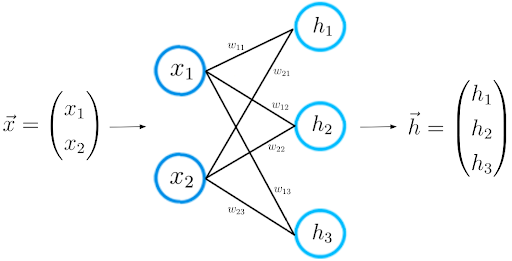
\includegraphics[width=0.8\textwidth]{slike/proces.png}
    \caption{Širenje; prema: \cite{builtin1}}
    \label{fig:proces}
\end{figure}

\newpage
\blockquote[{\cite{builtin1}}]{Na slici \ref{fig:proces} se prikazuje proces širenja unaprijed. Koristeći ulazni vektor $x$ i matricu vrijednosti $W$ koja povezuje dva sloja neurona, izračunava se skalarni produkt između vektora $x$ i matrice $W$.
Rezultat ovog skalarnog produkta je drugi vektor, nazvan $z$.

\[
\begin{aligned}
\vec{x}^T \cdot W &=\left(x_1, x_2\right) \cdot\left(\begin{array}{lll}
w_{11} & w_{12} & w_{13} \\
w_{21} & w_{22} & w_{23}
\end{array}\right) \\
&=\left(x_1 w_{11}+x_2 w_{21}, x_1 w_{12}+x_2 w_{22}, x_1 w_{13}+x_2 w_{23}\right) \\
&=\left(z_1, z_2, z_3\right)=\vec{z}, \vec{h}=\sigma(\vec{z})
\end{aligned}
\]

Konačni vektor predviđanja $h$ dobiva se primjenom takozvane aktivacijske funkcije na vektor $z$. Aktivacijska funkcija je označena slovom $\sigma$ i ona predstavlja nelinearnu funkciju koja izvodi nelinearno preslikavanje iz $z$ u $h$.}
Jačina veze \cite{builtin1} između neurona iskazuje se kao linearna kombinacija težinskih vrijednosti povezanih neurona iz prethodnog sloja, u odnosu na promatrani neuron.

\subsection{Konvolucijske neuronske mreže}

Konvolucijska neuronska mreža (\textit{CNN}, eng. \textit{Convolutional Neural Network}) \cite[str. 326]{deep} je specijalizirana vrsta neuronskih mreža za za pretprocesiranje nestrukturiranih podataka, posebice vezanih za slike, tekst, zvuk i govor. Primjerice, \textit{CNN}-ovi imaju ponavljajuće slojeve neurona koji se primjenjuju u prostoru (za slike) ili vremenu (za audio signale, itd.). Za slike, ti neuronski slojevi mogu se tumačiti kao 2D konvolucijske jezgre koje se ponavljajući primjenjuju na svaki dio slike. Za govor, oni se mogu promatrati kao 1D konvolucijske jezgre.

\textit{CNN}-ovi su posebno korisni za pronalaženje uzoraka u slikama za prepoznavanje predmeta, lica i scene. Oni također mogu biti vrlo učinkoviti u klasificiranju neslikovitih podataka kao što su audio, vremenske prognoze i signalni podaci.

Kada je riječ o pronalaženju uzoraka iz slika, konvolucijske neuronske mreže mogu imati desetke ili stotine slojeva (Slika \ref{fig:konvolucija} i \ref{fig:konvmreza} ), od kojih svaki uči otkrivati različite značajke slike. Filtri se primjenjuju na svaku sliku za obuku u različitoj razlučivosti, a izlaz svake modificirane slike koristi se kao ulaz za sljedeći sloj. Filtri mogu započeti s vrlo jednostavnim značajkama, kao što su svjetlina i rubovi i dodati složenost kako bi se jedinstveno definirale karakteristike objekta \cite[str. 90]{fundamentals}.

Postoje četiri glavna koraka \cite{konv} u izvođenju operacija koji mijenjaju podatke s ciljem učenja značajki specifičnih za podatke: konvolucija, \textit{ReLU} (eng. \textit{Rectified Linear Unit}) aktivacijska funkcija i potpuna povezanost. 

\begin{figure}[!ht]
    \centering
    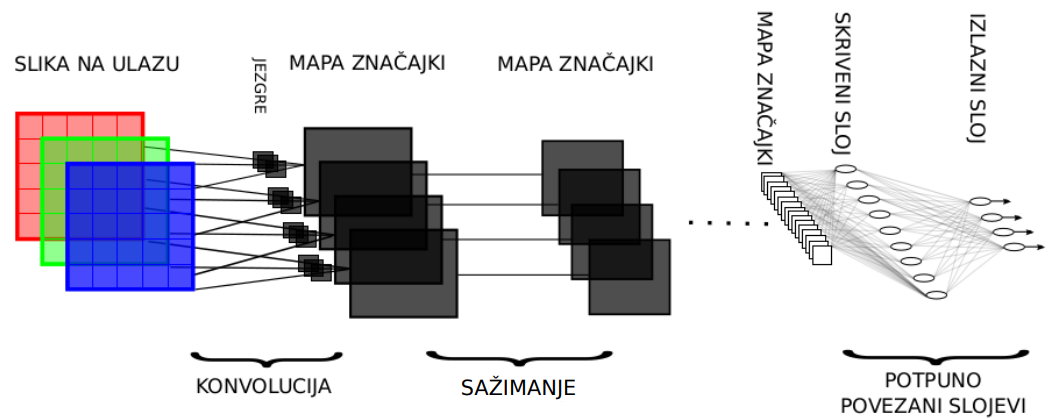
\includegraphics[width=1\textwidth]{slike/konvolucija.png}
    \caption{Arhitektura konvolucijske neuronske mreže; prema: \cite{builtin1}}
    \label{fig:konvolucija}
\end{figure}

Prvi sloj koji prima ulazni signal naziva se konvolucijski filtar. Konvolucija (eng. \textit{Convolution}) \cite[str. 327]{deep} je proces u kojem mreža pokušava označiti ulazni signal pozivajući se na ono što je naučila u prošlosti. Primjerice, ako ulazni signal izgleda kao slika mačke koja je već viđena, referentni signal "mačke" bit će pomiješan ili konvolviran s ulaznim signalom. Rezultirajući izlazni signal zatim se prosljeđuje sljedećem sloju.
Sažimanje (eng. \textit{pooling}) \cite{konv} pojednostavljuje izlaz izvođenjem nelinearnog smanjivanja uzorkovanja, smanjujući broj parametara koje mreža mora naučiti (Slika \ref{fig:primjer}).

\begin{figure}[!ht]
    \centering
    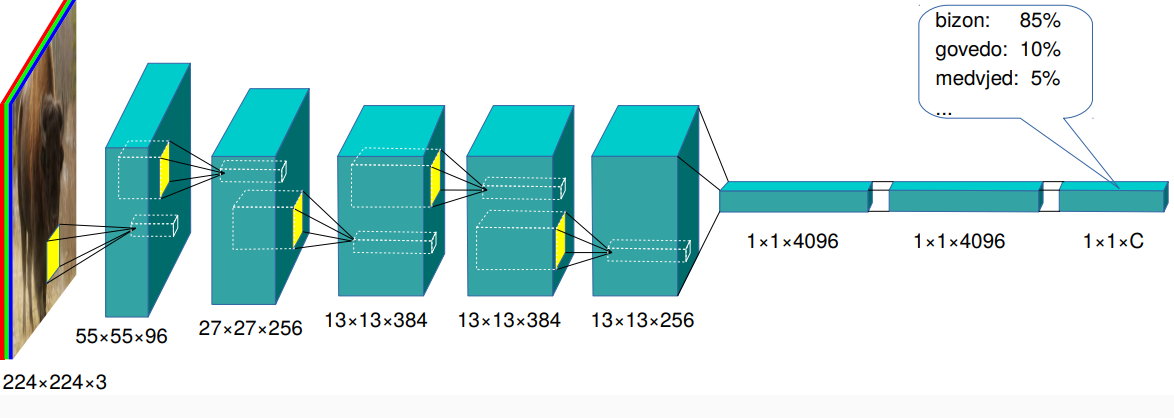
\includegraphics[width=1\textwidth]{slike/primjer.png}
    \caption{Praktični primjer na temelju prepoznavanja životinje: bizona, goveda i medvjeda; prema: \cite{konv}}
    \label{fig:primjer}
\end{figure}

Potpuno povezani (eng. \textit{Fully Connected (FC)}) \cite[str. 89, 90]{fundamentals} slojevi su slojevi gdje je svaki ulaz povezan sa svim neuronima. Ako postoje, potpuno povezani slojevi obično se nalaze blizu kraja \textit{CNN} arhitekture i mogu se koristiti za optimizaciju ciljeva kao što su rezultati razreda.

Aktivacijska funkcija (\textit{ReLU} (eng. \textit{Rectified Linear Unit})) \cite[str. 13-15]{fundamentals} omogućava bržu i učinkovitiju obuku preslikavanjem negativnih vrijednosti na nulu i zadržavanjem pozitivnih vrijednosti. To se ponekad naziva aktivacijom jer se samo aktivirane značajke prosljeđuju na sljedeći sloj.

\begin{figure}[!ht]
    \centering
    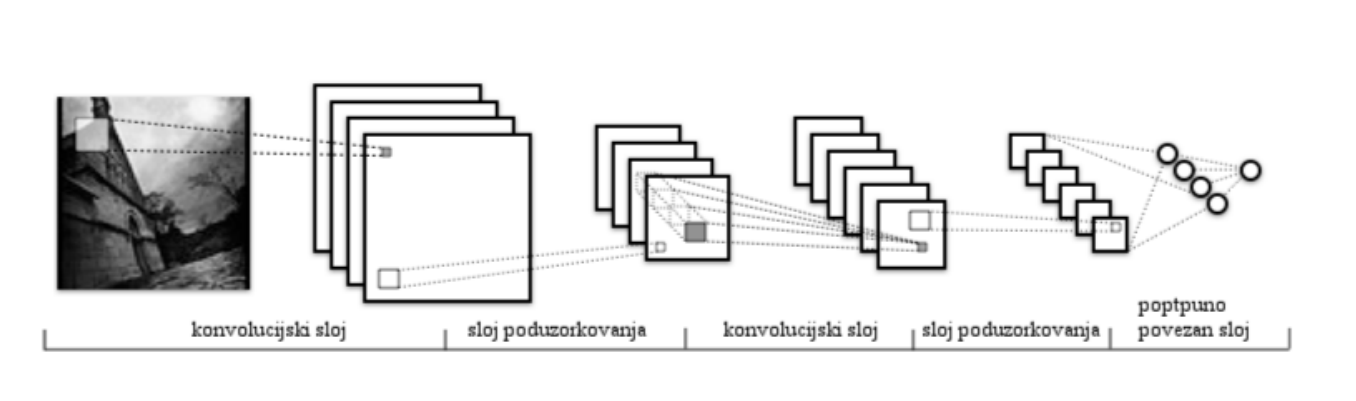
\includegraphics[width=1\textwidth]{slike/konvmreza.png}
    \caption{Slojevi konvolucije, poduzorkovanja i potpuno povezani sloj; prema: \cite{konv}}
    \label{fig:konvmreza}
\end{figure}

Jedan od primjera primjene konvolucijskih mreža su aplikacije \cite{primjena} za pretvaranje govora u tekst kod kojih je najbitnija stvar otkrivanje ključnih riječi. Dakle, aplikacija identificira određene ključne riječi ili fraze i može ih koristiti kao upute.

Još jedan primjer \cite{primjena} korištenja \textit{CNN}-ova je za semantičku segmentaciju gdje se identificira svaki piksel na slici s odgovarajućom oznakom klase. Semantička segmentacija može se koristiti u aplikacijama kao što su autonomna vožnja, industrijska inspekcija, klasifikacija terena i medicinsko snimanje. Konvolucijske neuronske mreže osnova su za izgradnju semantičkih segmentacijskih mreža.

\chapter{Računalni vid}

Ljudi su desetljećima sanjali o stvaranju strojeva s karakteristikama ljudske inteligencije, odnosno strojeva koji mogu razmišljati i ponašati se poput ljudi. Jedna od najfascinantnijih ideja je omogućiti računalima da "vide" i tumače svijet oko sebe (Slika \ref{fig:einstein}). Tadašnja fantazija danas postaje stvarnost \cite[str. 3]{szeliskicvaa}.

Zahvaljujući napretku umjetne inteligencije i računalne snage, tehnologija računalnog vida napravila je velik korak prema integraciji u naš svakodnevni život.

Računalni vid je polje umjetne inteligencije \cite{wikipedia} koje omogućuje računalima i sustavima da izvuku značajne informacije iz digitalnih slika, videa i drugih vizualnih \textit{inputa} te da djeluju ili daju preporuke na temelju tih informacija. Ako umjetna inteligencija računalima omogućuje razmišljanje, računalni vid im omogućuje da vide, promatraju i razumiju.

Kao znanstvena disciplina \cite{wikipedia}, računalni vid bavi se teorijom iza umjetnih sustava (neuronskih mreža) koji dohvaćaju informacije iz slika. Podaci o slikama mogu imati mnoge oblike, kao što su video sekvence, prikazi s više kamera ili višedimenzionalni podaci iz medicinskih skenera.
Kao tehnička disciplina \cite{wikipedia}, računalni vid nastoji "primijeniti svoje teorije i modele na stvarni svijet" za dobrobit čovječanstva.

\vspace{10mm}
\begin{figure}[!ht]
    \centering
    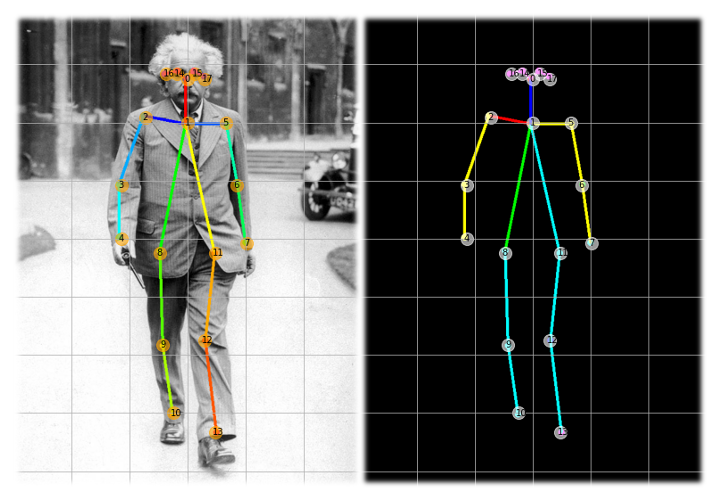
\includegraphics[width=0.75\textwidth]{slike/einstein.png}
    \caption{Primjer korištenja računalnog vida u stvarnom životu; prema: \cite{szeliskicvaa}}
    \label{fig:einstein}
\end{figure}

\newpage
\section{Pregled povijesti}

U ovom odjeljku sadržan je kratak pregled glavnih razdoblja razvoja računalnog vida tijekom posljednjih 50 godina (Slika \ref{fig:vremlinija}.) s naglaskom na napredak u razvoju algoritama i obradu podataka.

\begin{figure}[!ht]
    \centering
    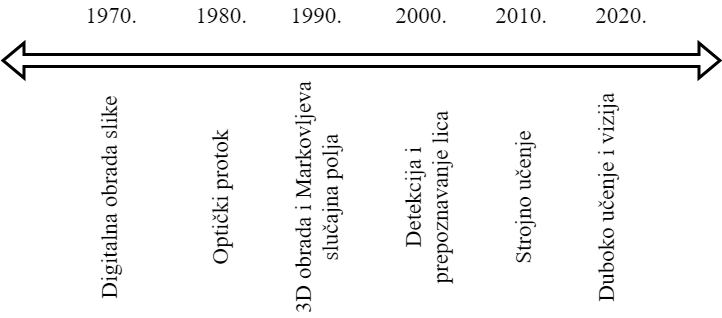
\includegraphics[width=0.87\textwidth]{slike/vremenskalinija.png}
    \caption{Vremenski raspored odabranih tema istraživanja u računalnom vidu; prema: \cite{szeliskicvaa}}
    \label{fig:vremlinija}
\end{figure}

\begin{figure}[!ht]
    \centering
    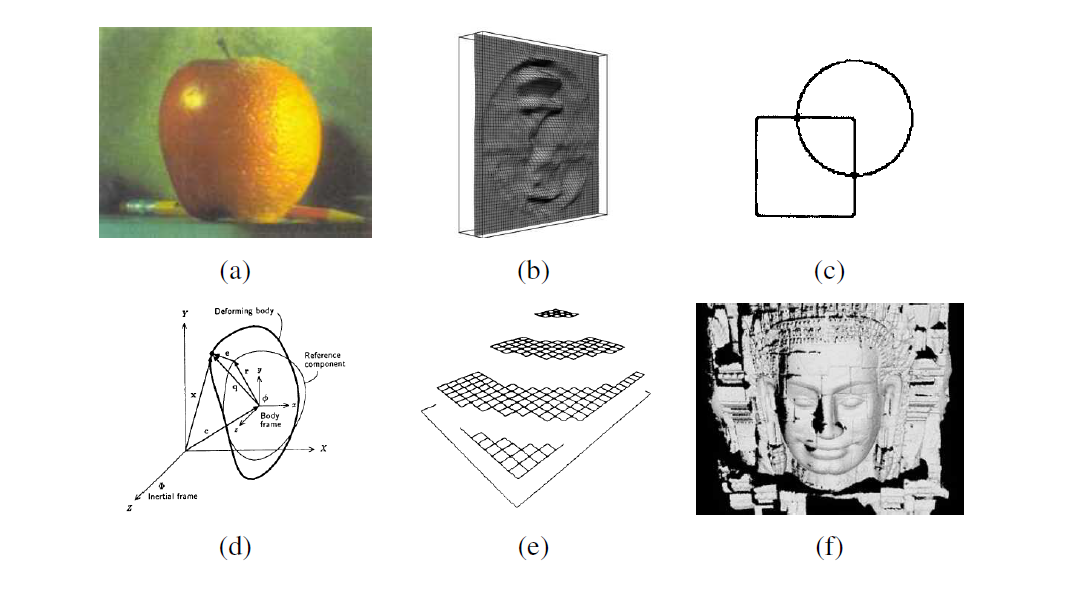
\includegraphics[width=1.1\textwidth]{slike/1980.png}
    \caption{Primjeri algoritama računalnog vida iz 1980-ih: (a) piramidalno spajanje, (b) oblik iz sjenčanja, (c) otkrivanje rubova, (d) fizički bazirani modeli, (e) površinska rekonstrukcija temeljena na regularizaciji, (f) prikupljanje podataka o rasponu; prema: \cite{szeliskicvaa}}
    \label{fig:1980ih}
\end{figure}

Pojava računalnog vida 70-ih godina 20. stoljeća \cite[str. 11]{szeliskicvaa} smatrala se jednostavnim rješenjem za znatni napredak same inteligencije stroja. Nastajući kao metoda oponašanja ljudske inteligencije \cite[str. 11]{szeliskicvaa}, računalni vid se u početku znatno podcjenjivao. Smatralo se kako za vid nije potrebna inteligencija, implementiranje softvera za vid bi trebalo biti intuitivno. Među prvim znanstvenicima koji je shvatio samu težinu izazova bio je i Marvin Minsky. Naime, u 1966. godini, Minsky je zajedno s bistrim studentom prve godine - Geraldom Sussmanom, proveo cijelo ljeto pokušavajući postići nekakav napredak \cite[str. 781]{minskySussman}. Generalna ideja bila je povezati računala s kamerama te ih navesti da opišu ono što vide. Iako su obojica bili vrlo optimistični, cijeli projekt je bio veliki neuspjeh, pokazalo se kako je razvoj takvog softvera iznimno kompliciran i problematičan. Samo polje računalnog vida i danas nakon nekoliko značajnih napredaka kaska za ljudskim vidom \cite{Huang1996ComputerVE}. Sposobnost čovjeka da prepoznaje mnogo lica, lica različite životne dobe u vrlo širokom spektru nepoželjnih uvjeta, teško da će i u skorom vremenu biti sustignuta.

Unutar narednog desetljeća pozornost se okrenula druge tipove problema. Glavni fokus 80-ih godina bile su složenije matematičke tehnike korištenih u analizi slika i scena \cite[str. 15]{szeliskicvaa}. Jedna od novih metoda je tzv. piramida slika (eng. \textit{image pyramid}) ili jednostavnije samo piramida. Piramida je metoda unutar koje su slika (ili signal) podložni izglađivanju (eng. \textit{smoothing}) i poduzorkovanju \textit{subsampling} \cite{wikipediaPiramida}. Do samog kraja desetljeća, obrada podataka nad 3D prostorima (prikupljanje, spajanje, modeliranje i identifikacija) bila je aktivno istraživana.

\begin{figure}[!hb]
    \centering
    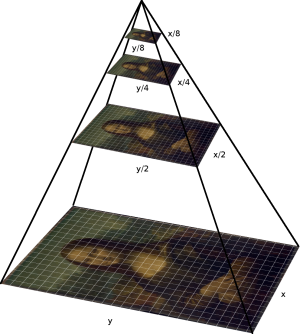
\includegraphics[width=0.68\textwidth]{slike/piramidaslika.png}
    \caption{Piramida slika; prema: \cite{szeliskicvaa}}
    \label{fig:piramidaSlika}
\end{figure}

Ovisno o vremenu, neke od spomenutih tema nastavljaju se naširoko razvijati 1990-ih godina. Jedan od problema koji su se nastojali riješiti bio je i problem pokreta (eng. \textit{motion problem}), odnosno procjene kretanja \cite[str. 15]{szeliskicvaa}. Ovaj problem središnji je dio mnogih projekata i radova i dan danas. U tom razvoju pokušane su tehnike poput projektivnih invarijanti (eng. \textit{projective invariants}), rekonstrukcija projekcije (eng. \textit{projective reconstructions}), tehnika faktorizacije (eng. \textit{factorization techniques}) i dr., no na kraju je uvedena uporaba potpune globalne optimizacije (eng. \textit{full global optimization}) \cite[str. 15-18]{szeliskicvaa}. Pomoću ove tehnike izgrađeni su potpuno automatizirani sustavi 3D modeliranja.

Može se reći kako razvoj računalnog vida prati i sami razvoj računala, pametnih uređaja, odnosno generalno tehnologije. Tako je početkom 21. stoljeća (Slika \ref{fig:2000ih}), točnije u prvom desetljeću 21. stoljeća, ubrzan razvoj grafike i vida. Izniman doprinos napretku je i prisutnost velikih skupova podataka (eng. \textit{big data}), no iako su oni prisutni, njihova prisutnost se kreće u potpunosti iskorištavati u narednom desetljeću. Najvažniji trend ovog desetljeća je primjena složenih tehnika strojnog učenja na probleme računalnog vida, kao što su neuronske mreže, nadzirano i nenadzirano učenje itd., koje su u potpunosti preuzele vizualno prepoznavanje i većinu drugih aspekata računalnog vida \cite[str. 19]{szeliskicvaa}.

\begin{figure}[!ht]
    \centering
    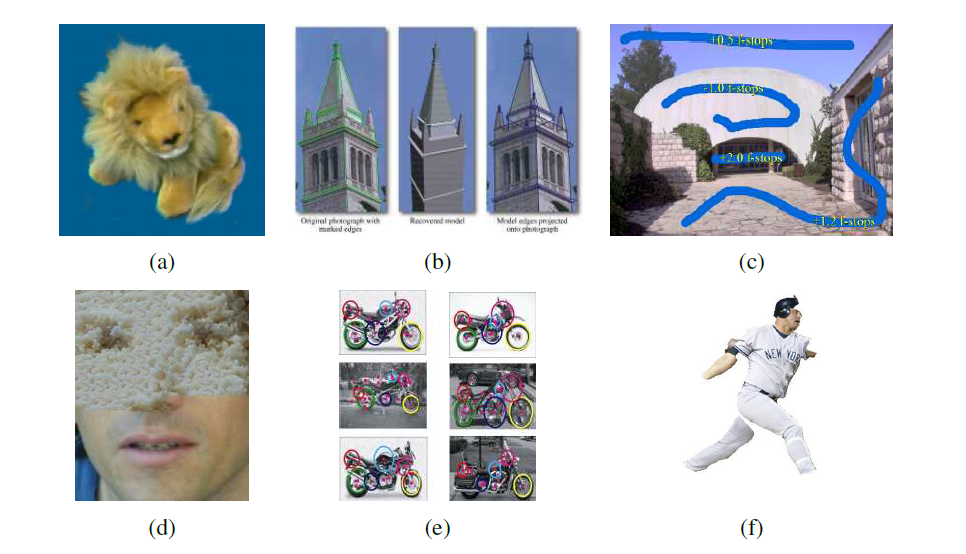
\includegraphics[width=1\textwidth]{slike/2000.png}
    \caption{Primjeri algoritama računalnog vida iz 2000-ih: (a) renderiranje, (b) modeliranje, (c) interaktivno preslikavanje tonova, (d) sinteza teksture, (e) prepoznavanje, (f) regionalno prepoznavanje; prema: \cite{szeliskicvaa}}
    \label{fig:2000ih}
\end{figure}

Zahvaljujući ogromnim napretcima unutar cijelog polja umjetne inteligencije, ali i susjednih polja poput znanosti o podacima, razvoj računalnog vida dosegnuo je nove visine. Po prvi puta u povijesti moguće je prikupiti, organizirati i spremiti ogromne količine skupova podataka. Zbog toga, novi trend koji se javlja 2010-ih godina, korištenje je velikih označenih skupova podataka čime se revolucionarizirao razvoj algoritama za prepoznavanje slika \cite[str. 20]{szeliskicvaa}. \textit{SLAM} (simultana lokalizacija i mapiranje, eng. \textit{Simultaneous Localization And Mapping}) i \textit{VIO} (vizualna inercijalna odometrija, eng. \textit{Visual Inertial Odometry)}) \cite[str. 20, 21, 22]{szeliskicvaa} poznati su algoritmi računalnog vida koji se koriste unutar naprednijih platforma poput dronova i autonomnih vozila \cite[str. 22]{szeliskicvaa}. Koristeći te algoritme moguće je izraditi točne 3D karte u stvarnom vremenu za, npr. autonomni let u izazovnim scenama kao što su šume ili urbana okolina. 

Ukratko rečeno, računalni vid razvijao se kroz zadnjih 50 godina uz razne uspone i padove. Početni zanos, entuzijazam i optimizam vrlo je brzo zamijenjen realnošću - računalni vid vrlo je složeno područje čija kompleksnost znatno sprječava veći napredak. Najveći napredak ostvaren je u prethodnom desetljeću zbog generalnog razvoja strojnog učenja, neuronskih mreža i drugih dijelova umjetne inteligencije. Zahvaljujući tome, računalni vid danas ima primjenu u mnogim dijelovima našeg života - od kamera u pametnim mobitelima, preko autonomnih vozila i prometa pa sve do medicine. Jednostavno rečeno, primjena je mnogo, a nastavkom razvoja mogućnosti će biti mnogo veće.

\newpage
\section{Digitalna obrada slike}

Prije analize i obrade slike potrebno je naglasiti određene pojmove koji opisuju obradu slike. Poanta je u tom da je potrebno razumjeti proces formiranja slike (Slika \ref{fig:formacija}) koji proizvodi određenu sliku s obzirom na skup uvjeta osvjetljenja, prostornu geometriju, svojstva površine i optiku kamere (Slika \ref{fig:matrica}).

\begin{figure}[!ht]
    \centering
    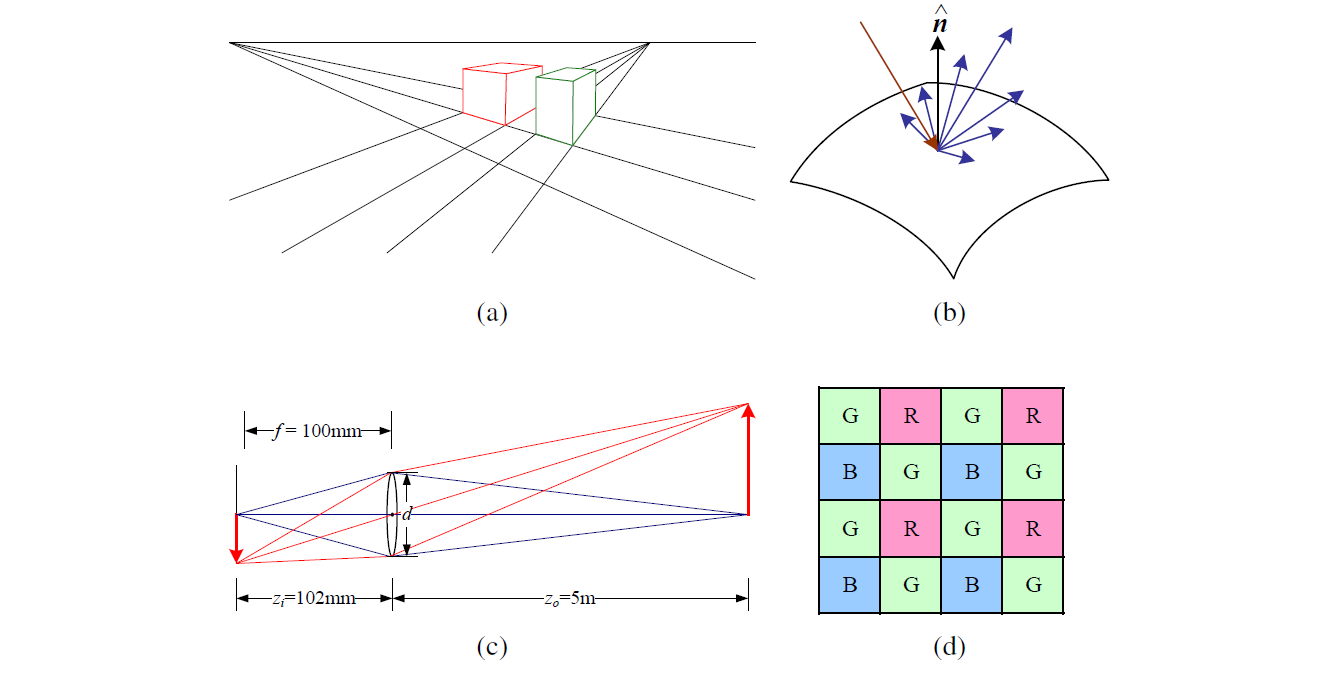
\includegraphics[width=1\textwidth]{slike/formacija.png}
    \caption{Komponente procesa oblikovanja slike: (a) perspektivna projekcija, (b) raspršenje svjetlosti pri udaru o površinu, (c) optika leća, (d) Bayerov niz filtera u boji; prema: \cite{szeliskicvaa}}
    \label{fig:formacija}
\end{figure}

\blockquote[{\cite{digital}}]{Slika, definirana matematičkim rječnikom, može se prikazati kao dvodimenzionalna funkcija, $F(x,y)$, gdje su $x$ i $y$ prostorne koordinate, a veličina $F$ je bilo koji par koordinata $(x,y)$ naziva se intenzitet slike u tom trenutku.
Drugim riječima, slike se mogu definirati 2D nizovima posebno raspoređenim u retke i stupce.
Digitalna slika sastoji se od konačnog broja elemenata, od kojih svaki ima određenu vrijednost na određenom mjestu. Ti se elementi nazivaju slikovni elementi, objektni elementi u slikama i pikseli. Od nabrojanih, pikseli se najčešće koriste za predstavljanje elemenata digitalnih slika.}

\noindent
Slike su, matematičkim zapisom, predstavljene kao matrice te zbog toga postoji sljedeći zapis \cite{digital}:
\[
f(x,y) = 
\begin{bmatrix}
f(0,0) & f(0,1) & f(0,2) & ... & f(0,N-1)\\
f(1,0) & f(1,1) & f(1,2) & ... & f(1,N-1)\\
. & . & . &  & .\\
. & . & . &  & .\\
. & . & . &  & .\\
f(M-1,0) & f(M-1,1) & f(M-1,2) & ... & f(M-1,N-1)\\
\end{bmatrix}.
\]

\begin{figure}[!ht]
    \centering
    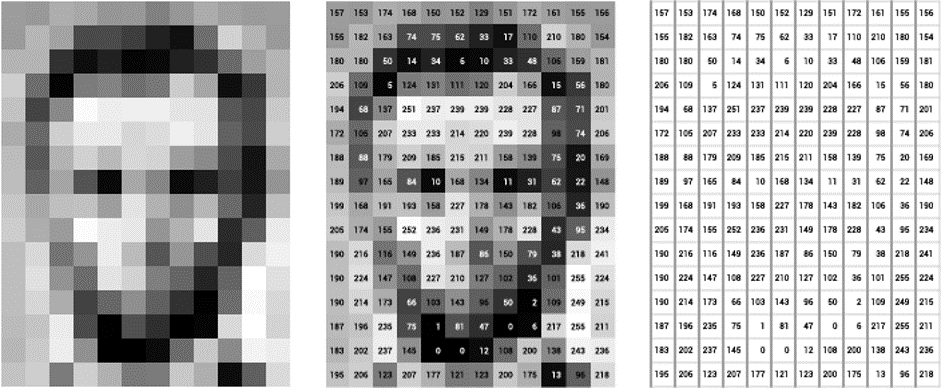
\includegraphics[width=0.9\textwidth]{slike/matrica.png}
    \caption{Vrijednosti boja pojedinačnih piksela; prema: \cite{adobe}}
    \label{fig:matrica}
\end{figure}

Kao što se može vidjeti na slici \ref{fig:dip} \cite{digital}, obrada slike podijeljena je na nekoliko znanstvenih područja na temelju slika (kao predmeta obrade) ili informacija kao ulaznih podataka \cite{digital}. Shodno tomu, može se reći da ako ulaz u proces obrade slike predstavlja sliku, tada je izlaz također slika jer se očekuje da taj proces nju obradi. Primjerice, poboljša njenu kvalitetu ili ju filtirira. Druga stvar, na primjer, ako za taj isti ulaz se opet stavi slika, a dobije se nekakva njena analiza, opis ili neki drugi tekstualni rezultat, tada se taj proces odvija pomoću računalnog vida. To znači da računalni vid analizira i daje rješenje u obliku opisa te slike. Primjerice, ulaz je bio slika psa, a proces je dao rezultat u tekstualnom obliku da je to pas. Nadalje, ako je sada obrnut proces, tj. ulaz je opis u tektualnom obliku ili kod, krajni rezultat slika, to se može nazvati računalnom grafikom jer je tu proces stvaranja odnosno prikaza slike iz date ulazne vrijednosti. I na kraju, ako se ulaz opet sastoji od nekakvog opisa ili programskog koda, a u ovom slučaju krajnji rezultat predstavlja opis ili analizu, onda se to može nazvati procesom koji je bio obrađivan uz pomoć umjetne inteligencije.

\begin{figure}[!ht]
    \centering
    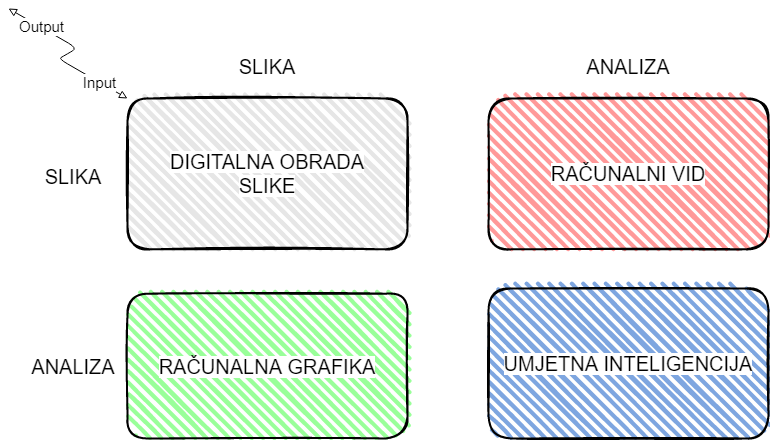
\includegraphics[width=0.9\textwidth]{slike/dip.png}
    \caption{Područja koja djeluju ovisno o slici ili vrsti informacije}
    \label{fig:dip}
\end{figure}

\newpage
\section{Prepoznavanje}

\begin{figure}[!ht]
    \centering
    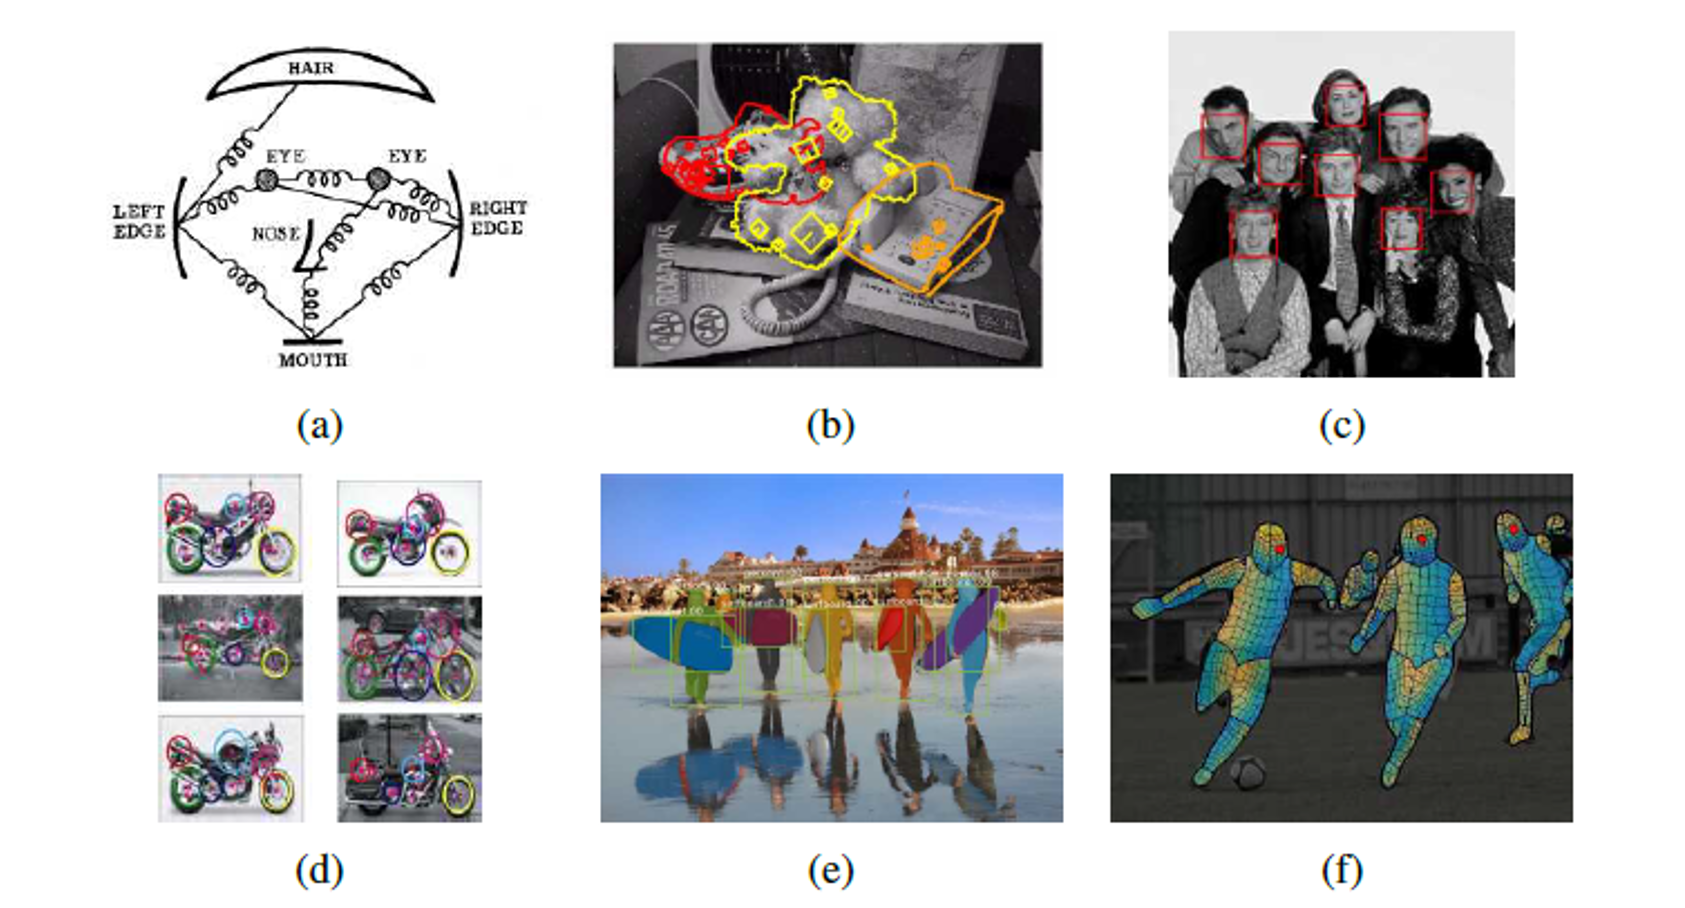
\includegraphics[width=1\textwidth]{slike/prepoznavanje.png}
    \caption{Razne vrste prepoznavanja: (a) prepoznavanje lica sa slikovnim strukturama, (b) prepoznavanje instanci (poznatog objekta), (c) prepoznavanje lica u stvarnom vremenu, (d) prepoznavanje temeljeno na značajkama, (e) segmentacija instance pomoću \textit{Mask} R-CNN, (f) procjena poze; prema: \cite{szeliskicvaa}}
    \label{fig:prepoznavanje}
\end{figure}

\subsection{Prepoznavanje objekata}

Prepoznavanje objekata opći je izraz koji se koristi za opisivanje povezanih zadataka računalnog vida koji uključuju prepoznavanje objekata na digitalnim fotografijama \cite[str. 349, 350]{szeliskicvaa}.
Kada osoba govori o "prepoznavanju predmeta" obično misli na "otkrivanje predmeta" (Slika \ref{fig:objekti}).
Klasifikacija slike uključuje predviđanje klase jednog objekta na slici. Lokalizacija objekta odnosi se na identificiranje lokacije jednog ili više objekata na slici i crtanje okvira oko njegovog opsega. Detekcija objekata kombinira ova dva zadatka za lociranje i klasificiranje jednog ili više objekata na slici.

Samo po sebi \cite[str. 346, 347, 349]{szeliskicvaa}, prepoznavanje objekata se može podijeliti na prepoznavanje instanci i prepoznavanje klase te kombinirati četiri tehnike: prepoznavanje slike, lokalizaciju objekta, detekciju objekta i segmentaciju slike. Prepoznavanje objekata analizira značajke slike i predviđa njezinu klasu ili kategorije putem klasifikatora, kao što je nadzirani model strojnog učenja primjerice, stroj potpornog vektora, \textit{Adaboost} algoritam, stabla odlučivanja. Prepoznavanje klasa kao područje istraživanja u prepoznavanju objekata znatno se brže razvija za razliku od tehnika prepoznavanja instanci koje svoju svrhu i dalje imaju u komercijalnim aplikacijama kao što je npr. prepoznavanje prometnih znakova, pješaka, semafora itd.

\begin{figure}[!ht]
    \centering
    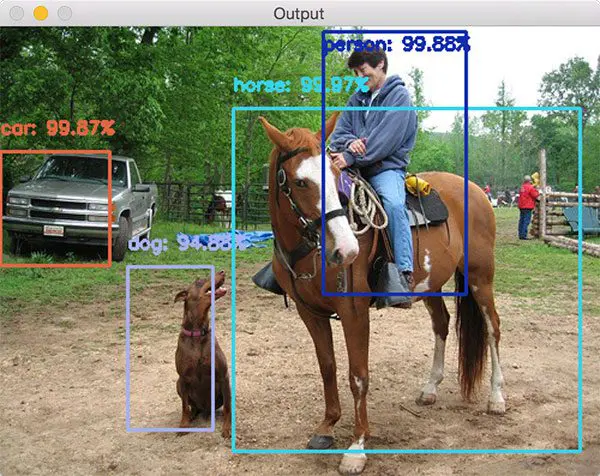
\includegraphics[width=0.5\textwidth]{slike/objekti.png}
    \caption{Detekcija okoline videokamerom; prema: \cite{szeliskicvaa}}
    \label{fig:objekti}
\end{figure}

\newpage
Regionalne konvolucijske neuronske mreže (\textit{R-CNN}, eng. \textit{Region-Based Convolutional Neural Network}) obitelj su tehnika za rješavanje zadataka lokalizacije i prepoznavanja objekata, dizajniranih za izvedbu modela \cite[str. 383, 385]{szeliskicvaa}. Metoda \textit{YOLO} (skraćeno od eng.\textit{You Only Look Once}) (Slika \ref{fig:yolo}) je klasa tehnika prepoznavanja objekata dizajniranih za brzu upotrebu u stvarnom vremenu. \textit{YOLO} \cite[str. 385]{szeliskicvaa} uključuje jednu neuronsku mrežu obučenu od kraja do kraja te uzima fotografije kao ulazne podatke i predviđa granične okvire i oznake klasa za svaki granični okvir. Ova tehnika inače pruža manju točnost predviđanja (npr. više pogrešaka lokalizacije), a iako ima brzinu promjene okvira u sekundi od 45 (\textit{fps}, eng. \textit{frames per second}), verzija modela koja je optimizirana, može postići brzinu i do 155 \textit{fps}-a.

\begin{figure}[!ht]
    \centering
    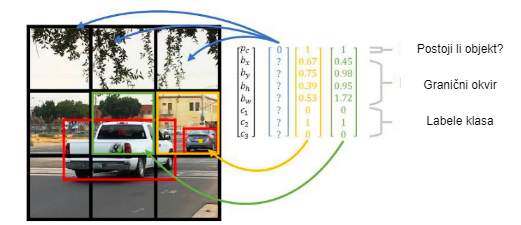
\includegraphics[width=1\textwidth]{slike/yolo.png}
    \caption{\textit{YOLO}, algoritam za otkrivanje objekata; prema: \cite{szeliskicvaa}}
    \label{fig:yolo}
\end{figure}

\newpage
\subsection{Prepoznavanje geste ruke}

Ljudska svakodnevnica ovih godina ne bi bila potpuna da nije napredovao razvoj računalnog vida \cite{hand3, hand1}. Primjerice, otključavanje mobilnih uređaja koristeći lice ili otisak prsta i sl. Među raznim tehnikama interakcije, korištenje ruku kao unosa je atraktivna metoda za uspostavljanje prirodne interakcije između čovjeka i računala. Korištenjem gesta korisnici npr. mobilnih uređaja mogu prenijeti više informacija u kraćem vremenu. Stoga, kako bi se poboljšalo sučelje između korisnika i računala, tehnologija interakcije između čovjeka i računala (\textit{HCI}, eng. \textit{Human–computer interaction}) ima veliku praktičnost \cite{hand3, hand1}.

Sustave za prepoznavanje specifičnih ljudskih gesti može se koristiti za prijenos bilo kakvih informacija ili kontrolu bilo kojeg uređaja ili robota u uredskim i kućnim aplikacijama. Statičko stanje ruke može se definirati kao poza dok dinamično se može definirati kao gesta koja predstavlja fizički pokret nekog od tjelesnih organa kao što su šake, ruke, lice itd. kako bi se prenijele značajne informacije, kao što su primjerice "lajk" ili "dislajk" \cite{hand1, hand2}. Za uspješnu komunikaciju, pošiljatelj i primatelj moraju imati slične informacije za određenu gestu. Postoje dvije uobičajene metode tumačenja gesta u interakciji između čovjeka i računala, a to su metoda temeljena na rukavicama baziranim na podacima i metoda temeljena na viziji \cite{hand2}.

\begin{figure}[!ht]
    \centering
    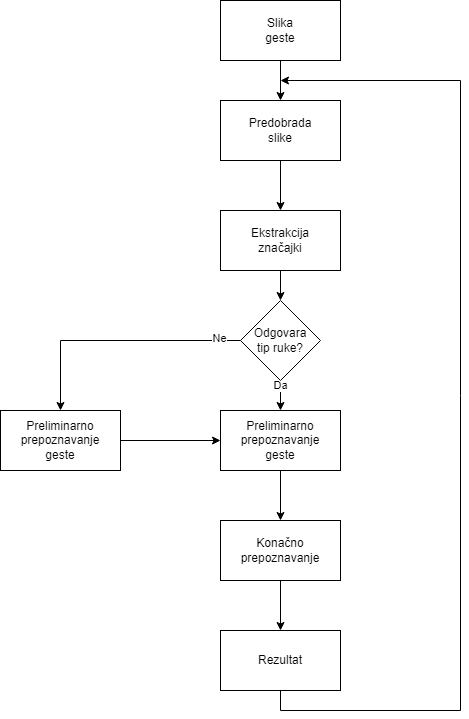
\includegraphics[width=0.55\textwidth]{slike/graf.png}
    \caption{Dijagram toka prepoznavanja}
    \label{fig:graf}
\end{figure}

\newpage
Tehnike detekcije ruku temeljene na značajkama koriste algoritme poput Viola-Jones algoritma i algoritma temeljenog na transformacijama značajki bez skaliranja \textit{SIFT (eng. Scale-Invariant Feature Transform)} \cite{hand2}. Ovi algoritmi daju rezultate visoke točnosti, ali su vrlo osjetljiviji na pozadinu. Jedan od ostalih pristupa za prepoznavanje gesta je algoritam \textit{AdaBoost} (eng. \textit{Adaptive Boosting}) koji integrira informacije iz iste klase objekata i obučava mrežu kombiniranjem svih slabih klasifikatora u jedan jak klasifikator \cite{hand1}. \textit{AdaBoost} algoritam učenja odabire najbolji slabi klasifikator iz skupa pozitivnih i negativnih uzoraka slike. Osim toga, algoritam daje rezultate s većom preciznošću i većom brzinom, ali ponekad zahtijeva više vremena za obuku mreže.

\vspace{10mm}
\begin{figure}[!ht]
    \centering
    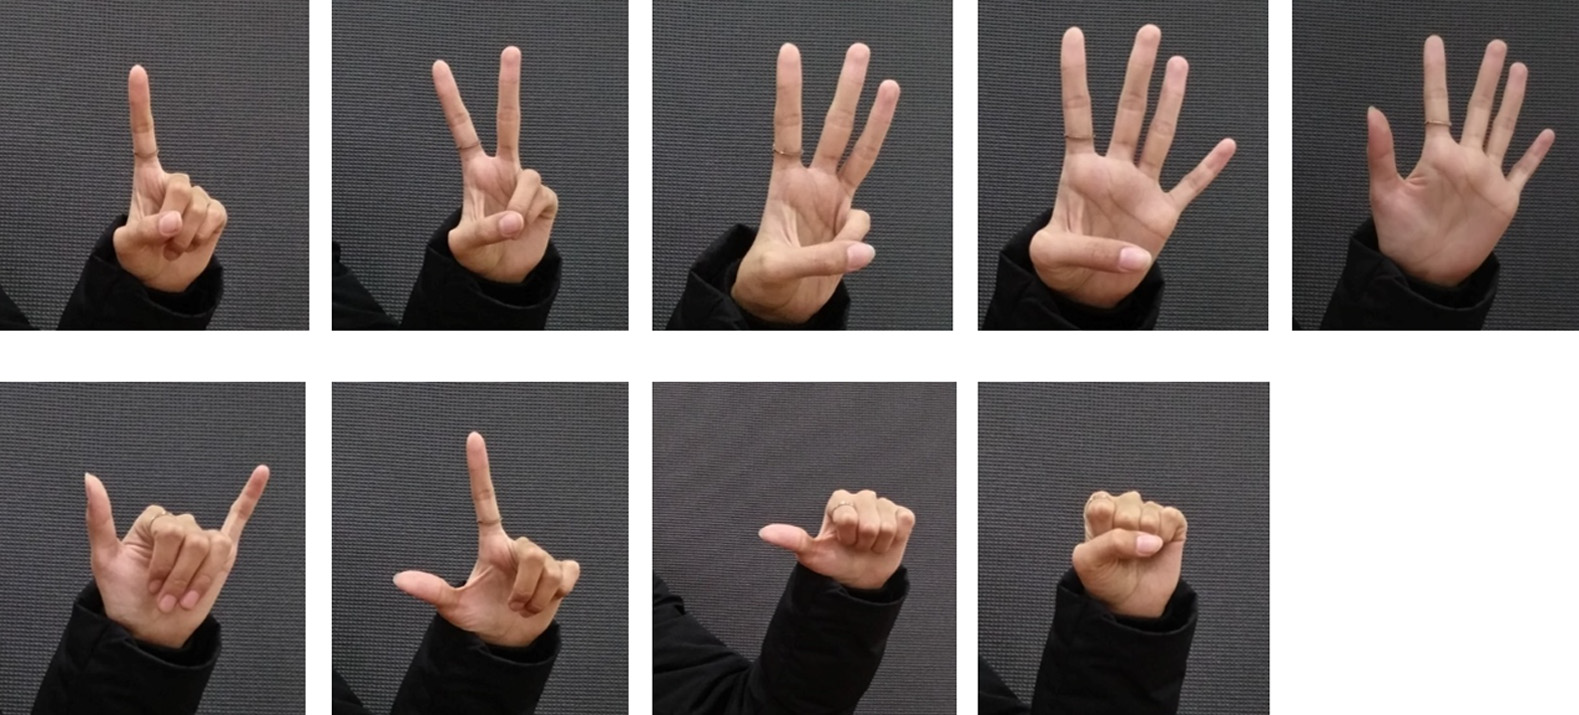
\includegraphics[width=1\textwidth]{slike/geste.png}
    \caption{Geste ruke; prema: \cite{hand4}}
    \label{fig:geste}
\end{figure}
\vspace{10mm}

Koraci obrade klasifikacije gesta \cite{hand2} uključuju prikupljanje gesta (Slika \ref{fig:geste}), segmentaciju, filtriranje, predstavljanje kontura i klasifikaciju korištenjem različitih tehnika. Prema dijagramu toka prepoznavanja ruke (Slika \ref{fig:graf}) prelazi se na primjenjeni dio gdje se analizira dlan ruke te uz pomoć točki označenih na rubovima prstiju se pokušava detektirati ruka. Najupečatljivija linija je ona gdje se duljina dlana, označena kao $L_1$, uzima od vrha najdužeg prsta do samog dna dlana. Zatim se mjeri duljina najdužeg prsta $L_2$ od vrha pa do njegovog dna. I za kraj se mjeri širina dlana koja je označena s $L_3$.

\begin{figure}[!ht]
    \centering
    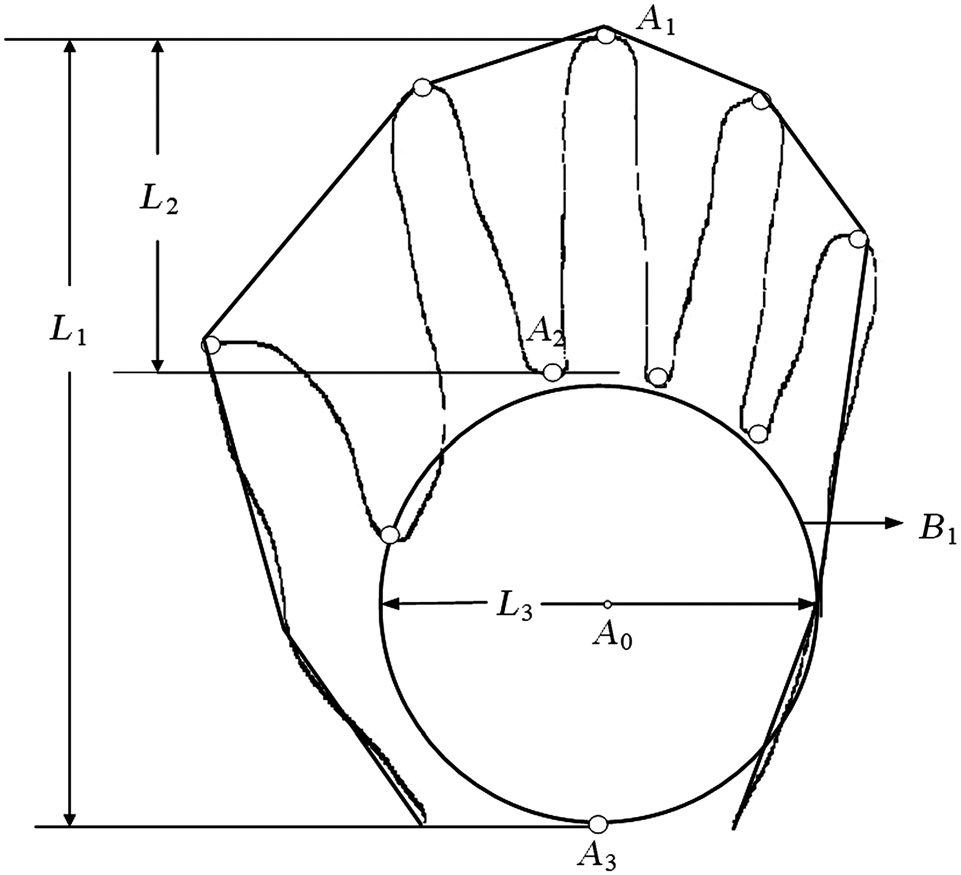
\includegraphics[width=0.6\textwidth]{slike/saka.png}
    \caption{Dijagram mjerenja duljine dlana; prema: \cite{hand4}}
    \label{fig:saka}
\end{figure}

\newpage
Na temelju prethodnih mjerenja (Slika \ref{fig:saka}), određuju se relativni položaji dlana i prstiju. $A_1$ predstavlja ordinatu vrha srednjeg prsta, $A_2$ najnižu točku srednjeg prsta zatim $A_3$ točku dna dlana te $A_0$ točku u središtu dlana. $L_1$, $L_2$ i $L_3$ izračunavaju se na sljedeći način \cite{hand4}:

\[
\left\{ \begin{array}{rcl} 
                L_1 = A_1 - A_3\\ 
                L_2 = A_1 - A_2 \\
                L_3 = 2 \times (A_0-A_3)
        \end{array}\right.
\]

U ovoj sekciji obrađivane su samo slike gesta dlana dok neki ostali dijelovi, npr. šaka ruke, nisu obrađeni. Slike gesta se filtriraju u fazi predobrade slike, kao što je prikazano na grafu \ref{fig:graf}, a zatim se pretvaraju iz RGB prostora boja u YCbCr prostor boja. S obzirom na to da tonovi boje kože imaju dobro grupiranje u YCbCr prostoru boja, može se postići segmentacija gesta \cite{hand4}. I na kraju se postiže sami rezultat, odnosno \textit{output} koji je dobiven postupkom konačnim prepoznavanjem.

\newpage
\section{Primjena}

Slikovite informacije imaju ključnu ulogu u medicinskoj dijagnozi jer čine gotovo većinu medicinskih i zdravstvenih informacija \cite{adobe}. Upravo zato, veliki broj dijagnoza temelji se na obradama medicinskih slika poput rendgenskih snimaka, magnetskih rezonanci i mamografija \cite{adobe}. Segmentacija slike je također pokazala svoju učinkovitost u analizi medicinskih skeniranja. Na primjer \cite{adobe}, algoritmi računalnog vida mogu otkriti dijabetičku retinopatiju, najbrže rastući uzrok sljepoće. Računalni vid može obraditi slike stražnjeg dijela oka (Slika \ref{fig:oko}) i procijeniti prisutnost i ozbiljnost bolesti.

\begin{figure}[!ht]
    \centering
    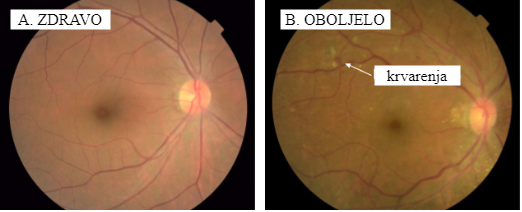
\includegraphics[width=0.9\textwidth]{slike/oko.png}
    \caption{Primjeri fotografija retinalnog fundusa. Slika s lijeve strane je zdrava mrežnica (A), dok je slika s desne strane mrežnica s dijabetičkom retinopatijom (B) zbog brojnih krvarenja (crvenih mrlja); prema: \cite{google1}}
    \label{fig:oko}
\end{figure}

\begin{figure}[!ht]
    \centering
    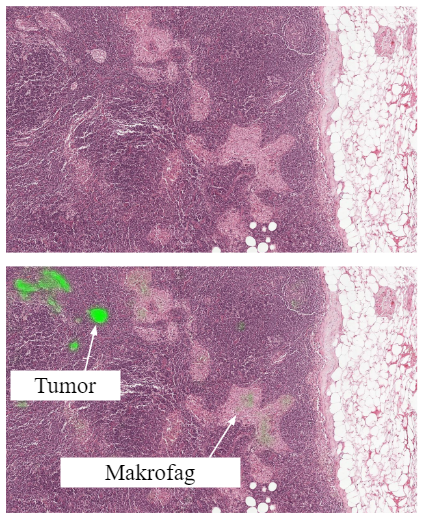
\includegraphics[width=0.45\textwidth]{slike/tumor.png}
    \caption{Krupni plan biopsije limfnog čvora; prema: \cite{google2}}
    \label{fig:tumor}
\end{figure}

Može se istaknuti kako je preciznost u dijagnosticiranju različitih oblika raka je ključna. Alati za računalni vid mogu otkriti metastaze raka ponekad točnije i od liječnika, sudeći prema \cite{google2}. Na slici \ref{fig:tumor} prikazan je krupni plan biopsije limfnog čvora čije tkivo sadrži metastaze raka dojke i područja koja izgledaju poput tumora, ali su dobroćudna. \cite{google2} Algoritam računalnog vida uspješno je identificirao područja tumora (svijetlozeleno) i nisu ga zbunila normalna područja koja su izgledala kao tumori.

Osim medicine, računalni vid omogućuje i automobilima razumijevanje okoline. Pametno vozilo \cite{adobe} u svom sustavu ima popriličan broj kamera koje mogu pratiti iz različitih kutova i slati sliku kao ulaz softveru za računalni vid. Sustav obrađuje sliku u stvarnom vremenu i otkriva oznake na cesti, objekte u blizini automobila (kao što su pješaci ili drugi automobili), semafore i još mnogo toga. Jedan od najvažnijih primjera primjene ove tehnologije je Teslin automobil.
Prema \cite{tesla}, autopilot predstavlja napredni sustav pomoći vozaču koji povećava sigurnost i udobnost vožnje. Kada (i ako) se pravilno koristi, autopilot može smanjiti opterećenje vozača. Svako novo Teslino vozilo (Slika \ref{fig:tesla}) opremljeno je s osam vanjskih kamera i snažnom vizualnom obradom za dodatni sloj sigurnosti. Sva vozila većinom napravljena za sjevernoameričko tržište sada koriste "Tesla Vision" temeljen na kameri za pružanje mogućnosti gotovo samostalne vožnje.

\begin{figure}[!ht]
    \centering
    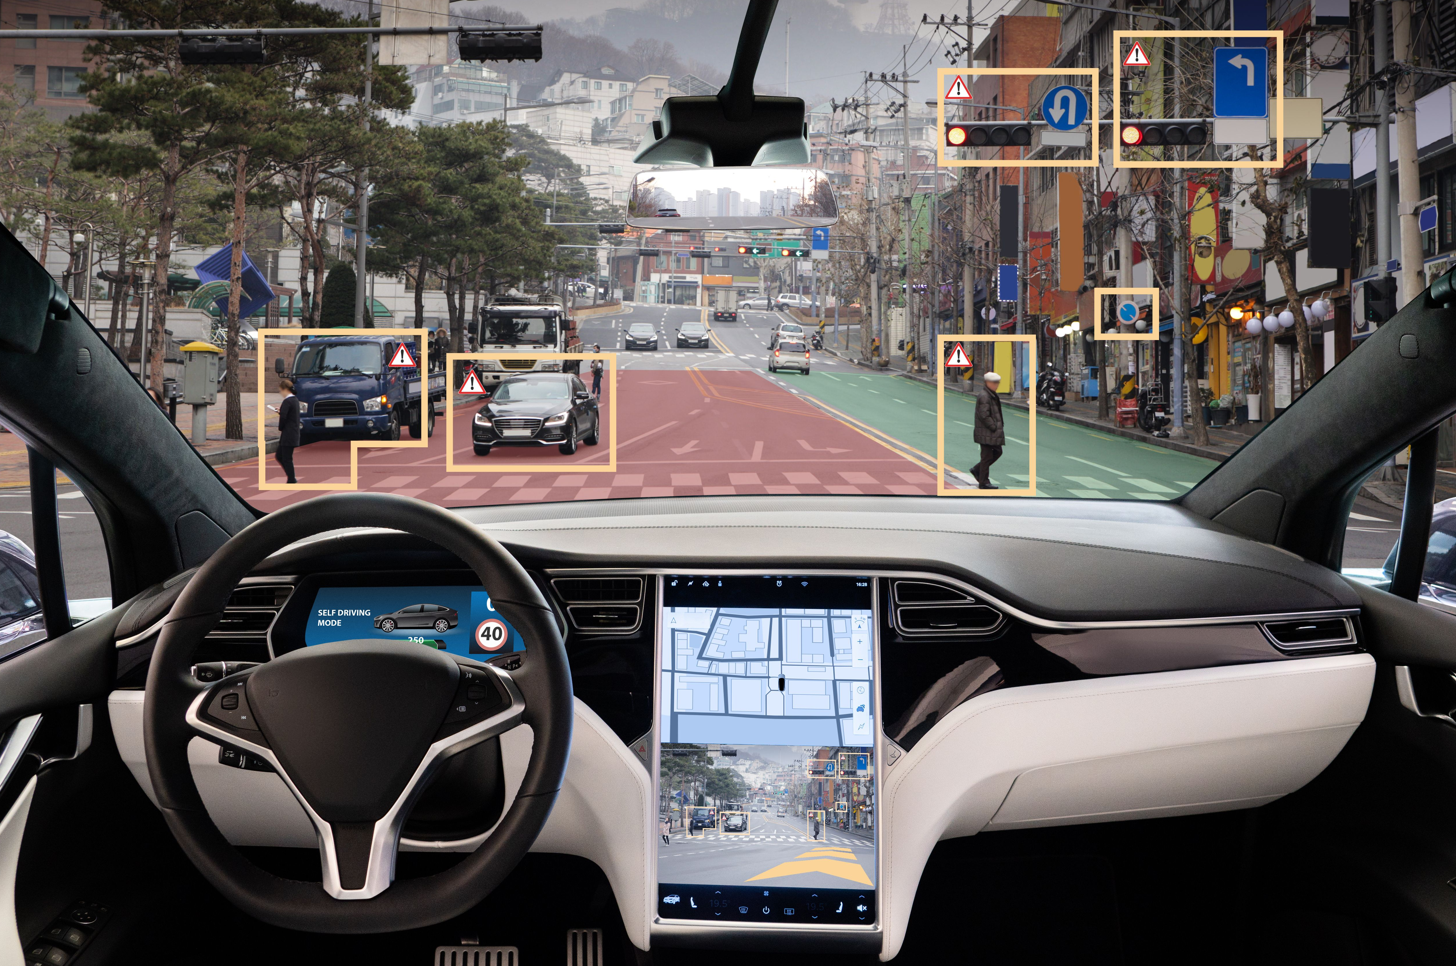
\includegraphics[width=0.6\textwidth]{slike/tesla.png}
    \caption{Unutrašnjost Tesla automobila te detekcija vanjskih objekata u prometu; prema: \cite{tesla}}
    \label{fig:tesla}
\end{figure}

Sve spomenuto o računalnom vidu također omogućuje poljoprivrednicima da se učinkovito bave većim površinama. Tehnologije poput dronova, senzora i satelitskih slika uz strojno učenje omogućavaju prikupljanje i analiziranje golemih količina podataka, što za rezultat ima, ne samo znatan napredak u količini i kvaliteti generiranih poljoprivrednih proizvoda, nego i u mnogim slučajevima spas poljoprivredne industrije \cite{vidhya}. Zahvaljujući prethodno spomenutim tehnologijama, mnogi poljoprivredni aspekti cjelokupnog procesa mogu biti i automatizirani. Osim toga, moguće ih je koristiti i u predviđanju prinosa te predviđanju i/ili identificiranju gubitaka uzrokovanih insektima, bolestima ili prirodnim uvjetima \cite{poljoprivreda}. Strojno učenje, odnosno računalni vid, danas moguće je koristiti i za rano otkrivanje i zaustavljanje biljnih bolesti \cite{vidhya}. Time se štedi vrijeme i novac, no najviše od svega stvara sigurnija i zdravija poljoprivredna praksa koja je iznimno podložna na vanjske, nepredvidive čimbenike.

\chapter{Implementacije praktičnog dijela}
\section{Opis i svrha}

Prepoznavanje gesta aktivno je područje istraživanja tehnologije interakcije čovjeka i računala. Ima mnoge primjene u kontroli virtualnog okruženja i prevođenju znakovnog jezika, kontroli robota, stvaranju glazbe itd. U ovom praktičnom dijelu dubokog učenja i računalnog vida o prepoznavanju gestikulacije rukama izradit će se implementacija prepoznavanja gestikulacija u stvarnom vremenu koristeći \textit{framework}-e odnosno biblioteke \texttt{MediaPipe}, \texttt{Tensorflow}, \texttt{OpenCV} i \texttt{Python}.

Nadalje, u drugoj implementaciji ovog praktičnog dijela rada, koristi se ruka kao virtualni miš za računalo koji može učiniti sve što i obični (fizički) miš za računalo, a da se ne dodirne sustav (tipkovnica, miš, \textit{touchpad}). Koristi se web kamera računala za otkrivanje ruku. Zatim će stvoriti okvir oko ruke i fokusirati se na dva prsta: kažiprst i srednji prst. Kažiprst će djelovati kao pokazivač i pomičući ga uokolo, pomicat će se pokazivač uokolo po zaslonu. Sada, kako bi se uspješno kliknulo pomoću detekcije ruke, bitna je udaljenost između kažiprsta i srednjeg prsta. Ako su spojeni zajedno ili na jako maloj udaljenosti, tada će se izvesti klik. Nadalje, dodan je faktor izglađivanja jer je pokret bio stvarno neusklađen.

\noindent
Za ispravan rad potrebno je instalirati sljedeće biblioteke:

\begin{itemize}
    \item \texttt{OpenCV},
    \item \texttt{MediaPipe},
    \item \texttt{Tensorflow},
    \item \texttt{AutoPy}.
\end{itemize}

\noindent
Ukratko su opisane sve od potrebnih biblioteka, a o \texttt{OpenCV} će biti govora malo kasnije.
\noindent
\texttt{MediaPipe} je biblioteka za izgradnju multimodalnih (npr. video, audio), međuplatformskih (tj. Android, iOS, web, perifernih uređaja) primijenjenih metoda strojnog učenja \cite{install}.

Može se instalirati pomoću "\texttt{pip install mediapipe}."

\noindent
\texttt{Tensorflow} je biblioteka za strojno učenje i duboko učenje kojeg je razvio tim Googlea. Može se koristiti u nizu zadataka, ali ima poseban fokus na duboke neuronske mreže \cite{install}.

Može se instalirati pomoću "\texttt{pip install tensorflow}."

\noindent
\texttt{AutoPy} je jednostavna biblioteka \textit{GUI} automatizacije za Python. Uključuje funkcije za upravljanje tipkovnicom i mišem, pronalaženje boja i bitmapa na zaslonu i prikaz upozorenja \cite{install}.

Može se instalirati pomoću "\texttt{pip install autopy}."

\noindent
Programski dio rada, rađen je \textit{Microsoft Visual Studio Code} okruženju.

\newpage
\section{OpenCV}

OpenCV (eng. \textit{Open Source Computer Vision Library}) \cite{opencv} biblioteka je softvera za računalni vid i strojno učenje otvorenog koda. OpenCV (Slika \ref{fig:opencv}.) je napravljen kako bi osigurao zajedničku infrastrukturu za aplikacije računalnog vida i ubrzao korištenje strojne percepcije u komercijalnim proizvodima. Budući da je proizvod s \textit{BSD} licencom, OpenCV tvrtkama olakšava korištenje i izmjenu koda.

Biblioteka ima više od 2500 optimizacijskih algoritama, uključujući velik broj klasičnih i najsuvremenijih algoritama računalnog vida i strojnog učenja. Ovi se algoritmi mogu koristiti \cite{opencv} za otkrivanje i prepoznavanje lica, identifikaciju objekata, klasificiranje ljudskog ponašanja u videozapisima, praćenje kretanja kamere, praćenje pokretnih objekata, izdvajanje 3D modela objekata, generiranje 3D oblaka točaka iz stereo kamera, spajanje slika za generiranje visoka rezolucija slike, pronalaženje sličnih slika iz baza podataka slika, uklanjanje crvenih očiju iz Flash slika, praćenje pokreta očiju, prepoznavanje krajolika i postavljanje markera za preklapanje proširene stvarnosti i još mnogo toga. OpenCV ima više od 47 tisuća korisnika zajednice i procjenjuje se da ima više od 18 milijuna preuzimanja. Knjižnicu naširoko koriste tvrtke, istraživačke grupe i vladine agencije.

Uz dobro etablirane tvrtke kao što su \textit{Google}, \textit{Yahoo}, \textit{Microsoft}, \textit{Intel}, \textit{IBM}, \textit{Sony}, \textit{Honda}, \textit{Toyota} koje koriste biblioteku, postoji mnogo \textit{startupova} kao što su \textit{Applied Minds, VideoSurf i Zeitera}, koji u velikoj mjeri koriste OpenCV \cite{opencv}. Upotreba OpenCV-a pri implementaciji uključuje spajanje slika uličnog prikaza, otkrivanje upada ili provala putem videonadzora, praćenje vozila, pomoć robotima u navigaciji, otkrivanje utapanja u bazenima, izvođenje interaktivne umjetnosti, pregled etiketa proizvoda u tvornicama diljem svijeta i brzo prepoznavanje lica.

Biblioteka sadrži \texttt{C++, Python, Java i MATLAB} sučelja i podržava \textit{Windows, Linux, Android i Mac OS}. OpenCV se uglavnom oslanja na aplikacije za viziju u stvarnom vremenu i koristi \textit{MMX} i \textit{SSE} upute kada su dostupne \cite{opencv}. Trenutno se aktivno razvijaju potpuno opremljena \textit{CUDA} i \textit{OpenCL} sučelja. Postoji preko 500 algoritama i oko 10 puta više funkcija koje podržavaju te algoritme \cite{opencv}. OpenCV je izvorno napisan u \texttt{C++} i ima predložak sučelja koji besprijekorno radi sa \texttt{STL} datotekama.\\ Može se instalirati pomoću "\texttt{pip install opencv-python}."


\begin{figure}[!ht]
    \centering
    
\includegraphics[width=0.6\textwidth]{slike/opencv.png}
    \caption{OpenCV i Python; prema: \cite{opencv}}
    \label{fig:opencv}
\end{figure}

\newpage
\section{Analiza korištenih metoda}

U obje implementacije koje slijede u nastavku, potrebno je uključiti biblioteke (kod \ref{lst:prvi}.) koje su bile u prethodnim poglavljima opisane, a koje su neophodne za rad.

\begin{lstlisting}[language=Python, caption={[Biblioteke] Biblioteke}, label=lst:prvi]
import cv2
import time
import math
import autopy
import numpy as np
import mediapipe as mp
import tensorflow as tf
from keras.models import load_model
\end{lstlisting}

Osim dosad spomenutih biblioteka, tu se nalaze i biblioteke \texttt{time}, \texttt{math} te \texttt{numpy} koje za svrhu ovog rada predstavljaju pomoćne biblioteke. Bitno je spomenuti kako za datoteku \texttt{virtualniMis.py} je potrebno uključiti modul \texttt{pracenjeRuke.py}. Upravo taj modul (kod \ref{lst:drugi}.) je jedan od ključnih elemenata izrade virtualnog miša jer se u njemu nalazi klasa (\texttt{detektorRuke}) koja sadrži neke od najbitnijih metoda za samu detekciju ruke prilikom prikaza u stvarnom vremenu.

\begin{lstlisting}[language=Python, caption={[Klasa detektorRuke] Klasa detektorRuke}, label=lst:drugi]
# uključivanje biblioteke zaglavlja za datoteku virtualniMis.py
import pracenjeRuke as pr
# klasa detektorRuke koja sadrži metode za detekciju ruke
class detektorRuke()
\end{lstlisting}

\begin{figure}[!ht]
    \centering
    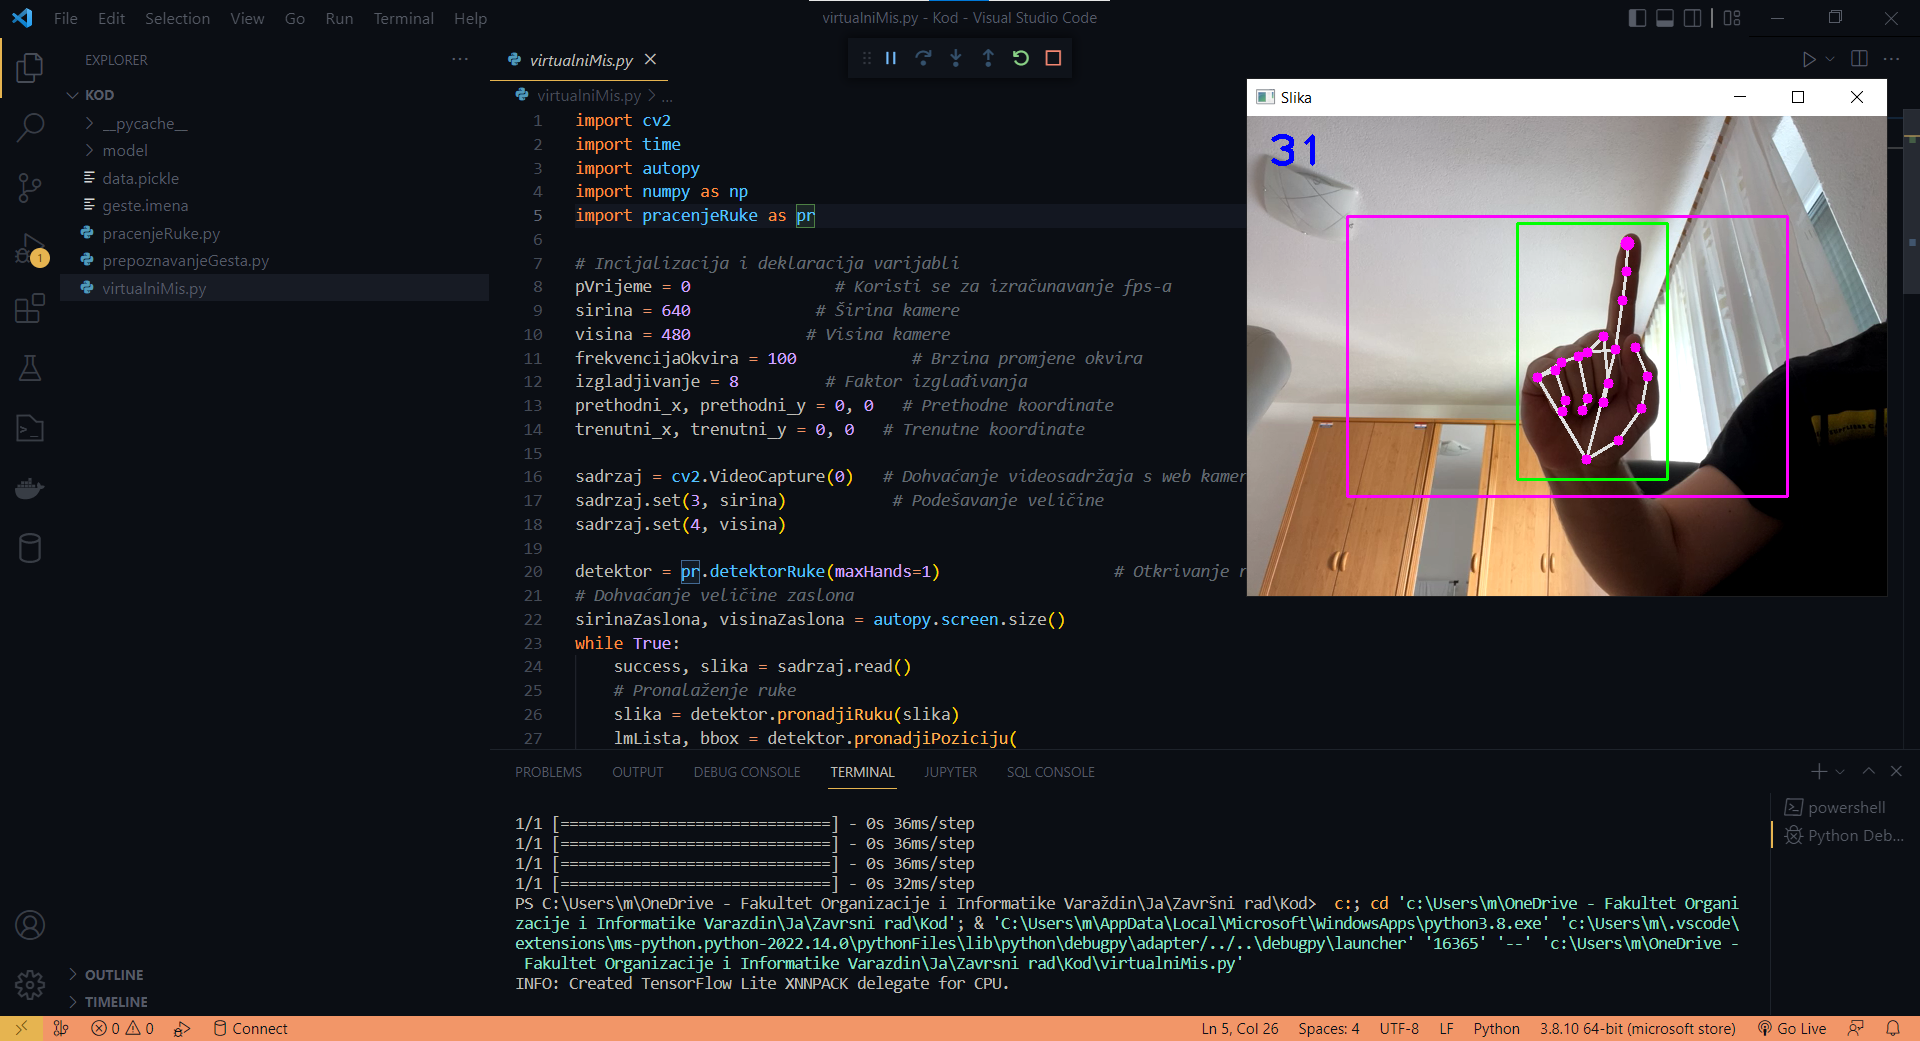
\includegraphics[width=0.8\textwidth]{slike/mis1.png}
    \caption{Pomicanje pokazivača po zaslonu}
    \label{fig:mis1}
\end{figure}

\newpage
Nadalje, metode klase \texttt{detektorRuke} koje je bitno spomenuti su:

\begin{itemize}
    \item \texttt{pronadjiRuku()} služi kako bi se detektirala ruka u određenom okviru te kako bi joj se dodijelili orijentiri koji bi se prikazali na ekranu.
    \item \texttt{pronadjiPoziciju()} služi za dohvaćanje položaja ruke, odnosno njene pozicije na slici.
    \item \texttt{prstPodignut()} služi za provjeravanje podignutog prsta, posebno za palac te posebno za ostale prste ruke.
    \item \texttt{pronadjiUdaljenost()} služi za pronalazak udaljenosti između kažiprsta i srednjeg prsta pomoću kojih se obavlja instrukcija "klika" na računalu.
\end{itemize}

\begin{figure}[!ht]
    \centering
    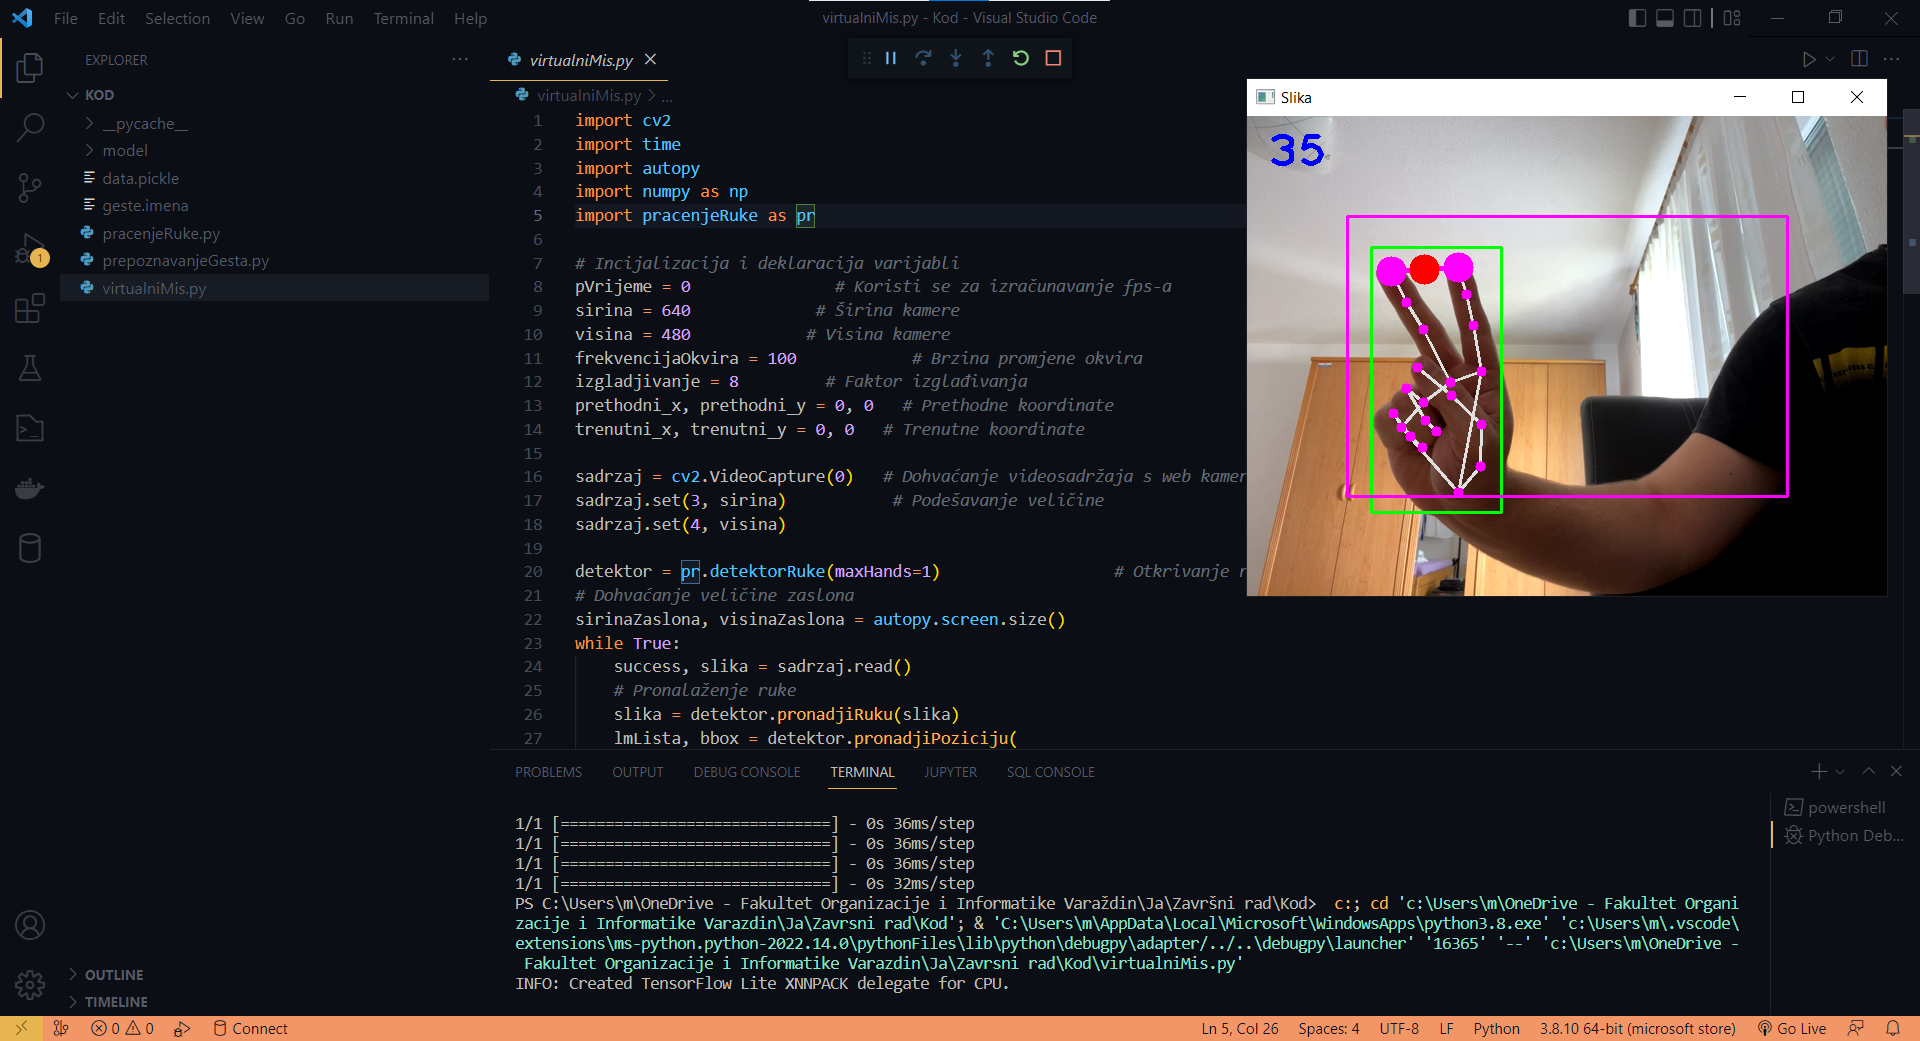
\includegraphics[width=0.8\textwidth]{slike/mis2.png}
    \caption{Klik}
    \label{fig:mis2}
\end{figure}

Datoteka \texttt{virtualniMis.py} predstavlja primarnu datoteku u kojoj se odvijaju operacije poput kretnje pokazivača po zaslonu (slika \ref{fig:mis1}.) te instrukcije klika gestikulacijom kažiprsta i srednjeg prsta (slika \ref{fig:mis2}).
Pomoću biblioteke \texttt{autopy} i njenih metoda \texttt{autopy.mouse.move()} i \texttt{autopy.mouse.click()} uspješno se izvršavaju instrukcije pomicanja pokazivača te klik (kod \ref{lst:treci}.) dohvaćajući trenutne informacije stečene gestikulacijom ruke.

\begin{lstlisting}[language=Python, caption={[Pomicanje pokazivača i klik] Pomicanje pokazivača i klik}, label=lst:treci]
# Pomicanje pokazivača
autopy.mouse.move(sirinaZaslona - trenutni_x, trenutni_y)
# Ako su kažiprst i srednji prst gore
if prsti[1] == 1 and prsti[2] == 1:     
    duljina, slika, linijaInfo = detektor.pronadjiUdaljenost(8, 12, slika)
# Ako su oba prsta jako blizu jedan drugome
if duljina < 40:
    cv2.circle(slika, (linijaInfo[4], linijaInfo[5]), 15, (0, 255, 0), cv2.FILLED)
# klik
    autopy.mouse.click()
\end{lstlisting}

Kod implementacije prepoznavanja gesti (\texttt{prepoznavanjeGeste.py}), najbitniju ulogu preuzima model. Model izvodi preciznu lokalizaciju svih ključnih 21 točaka 3D koordinate šake kao na slici \ref{fig:prsti}. i zgloba unutar detektiranih područja šake putem regresije, odnosno izravnog predviđanja koordinate. Model uči dosljedan interni prikaz položaja ruku i prikladan je čak i za djelomično vidljive ruke i samookluzije.

Kako bi se dobili istiniti podatci, ručno je označen veliki broj slika stvarnog svijeta s 3D koordinatama preko svih 21 označenih točaka, kao što je prikazano u nastavku (uzima se Z-vrijednost iz karte dubine slike, ako postoji po odgovarajućoj koordinati). Kako bi se bolje prikazali mogući položaji ruku i pružili dodatni provjeru nad prirodom geometrije ruku, renderira se visokokvalitetni sintetički model ruke preko različitih pozadina i mapira ga se na odgovarajuće 3D koordinate (Slika \ref{fig:rock}).

\begin{figure}[!ht]
    \centering
    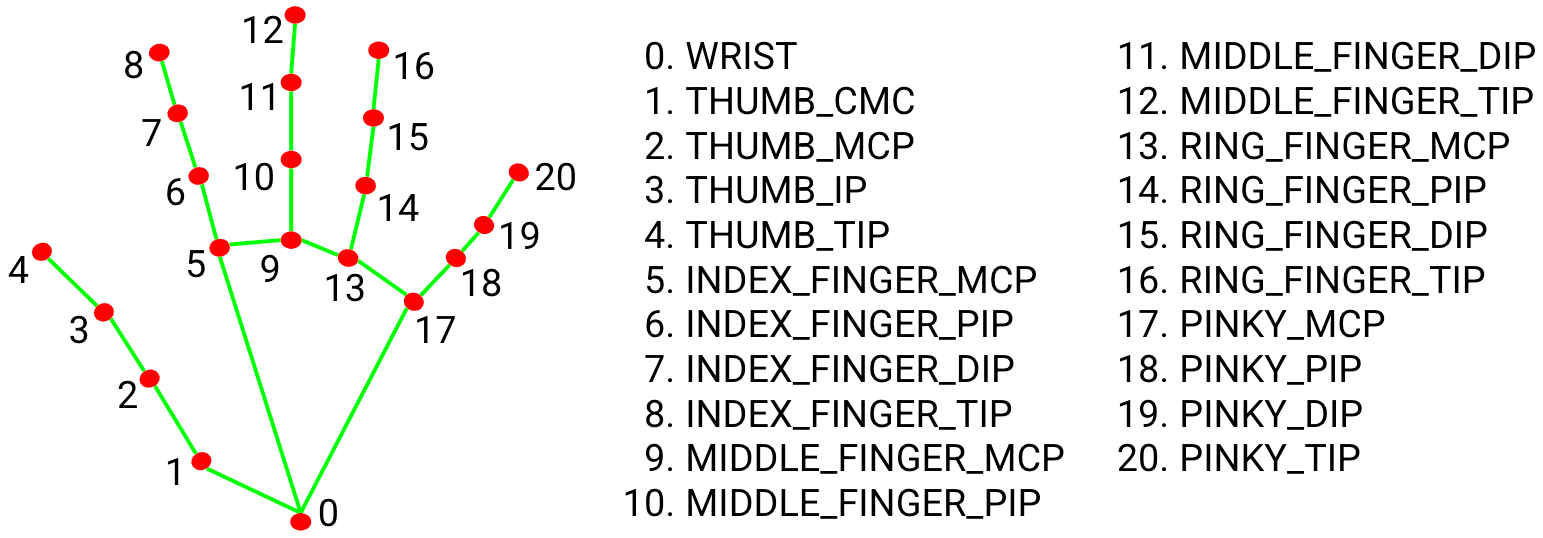
\includegraphics[width=0.8\textwidth]{slike/prsti.png}
    \caption{21 točka šake; prema: \cite{opencv}}
    \label{fig:prsti}
\end{figure}

Jedna od najbitnijih stvari za ovu implementaciju je inicijalizacija MediaPipe-a. (kod \ref{lst:cetvrti}). MediaPipeov modul \textit{mp.solution.hands} sadrži algoritam za prepoznavanje ruku. Stoga se prvo stvori objekt i pohrani ga u \textit{mpHands}.
Pomoću metode \textit{mpHands.Hands} se konfigurira model. Prvi parametar je \texttt{max\_num\_hands}, što znači da će model detektirati maksimalan broj ruku u okviru. MediaPipe može detektirati više ruku u jednom kadru, ali za sada je stavljeno da se detektira samo jedna po jedna ruku.
\texttt{Mp.solutions.drawing\_utils} odrađuje posao otkrivanja ključnih točki, tako da ih ne moramo crtati ručno.

\begin{lstlisting}[language=Python, caption={[Inicijalizacija MediaPipea] Inicijalizacija MediaPipea}, label=lst:cetvrti]
# Inicijalizacija MediaPipe-a.
mpHands = mp.solutions.hands
hands = mpHands.Hands(max_num_hands=1, min_detection_confidence=0.7)
mpDraw = mp.solutions.drawing_utils
\end{lstlisting}

\newpage
Pomoću funkcije \texttt{load\_model} se učitava unaprijed obučeni TensorFlow model (kod \ref{lst:peti}).
Datoteka \texttt{geste.imena} sadrži nazive klasa gesta. Prvo se ta datoteka otvori pomoću Python ugrađene funkcije \texttt{open()}, a nakon toga se koristi funkciju \texttt{read()} za čitanje datoteke.

\begin{lstlisting}[language=Python, caption={[Inicijalizacija TensorFlowa] Inicijalizacija TensorFlowa}, label=lst:peti]
# Učitavanje modela koji prepoznaje gestikulacije.
model = load_model('model')
# Učitavanje biblioteke naziva gestikulacija.
f = open('geste.imena', 'r')
imenaKlasa = f.read().split('\n')
f.close()
\end{lstlisting}

MediaPipe obrađuje RGB slike, ali OpenCV čita slike u BGR formatu. Pomoću funkcije \texttt{cv2.cvtCOLOR()} se sadržaj pretvara se u RGB format kako bi se vidjelo na zaslonu.

Zatim se koristi metoda \texttt{rezultat.multi\_hand\_landmarks} da provjeri jesu li prikazane ruke.
Nakon toga, ponavlja se svaka detekcija i spremaju se koordinate na popis koji se zove orijentir (eng. \textit{landmark}) (kod \ref{lst:sesti}.).
Ovdje se visina slike (y) i širina slike (x) množe s rezultatom jer model vraća normalizirani rezultat. To znači da je svaka vrijednost u rezultatu između 0 i 1.
Pomoću funkcije \texttt{mpDraw.draw\_landmarks()} prikazivaju se svi orijentiri u okviru. I na samom kraju, nakon pokazivanja ruke te detekcije geste, ostaje još samo prikazati dobiveni rezultat na zaslon pomoću metode \texttt{cv2.putText()}.

\begin{lstlisting}[language=Python, caption={[Prepoznavanje geste] Prepoznavanje geste}, label=lst:sesti]
if rezultat.multi_hand_landmarks:
    landmarks = []
    for handslms in rezultat.multi_hand_landmarks:
        for lm in handslms.landmark:
            #print(id, lm)
            lmx = int(lm.x * x)
            lmy = int(lm.y * y)

            landmarks.append([lmx, lmy])

        # Crtanje orijentira na prikazu.
        mpDraw.draw_landmarks(slika, handslms, mpHands.HAND_CONNECTIONS)

        # Predikcija gestikulacije.
        predikcija = model.predict([landmarks])
        # print(predikcija)
        klasaID = np.argmax(predikcija)
        imeKlase = imenaKlasa[klasaID]

# Prikazivanje predikcije.
cv2.putText(slika, imeKlase, (10, 50), cv2.FONT_HERSHEY_SIMPLEX, 1, (0, 0, 255), 2, cv2.LINE_AA)

cv2.imshow("Slika", slika)
\end{lstlisting}

\newpage
U ovim implementacijama prepoznavanja geste i virtualnog miša, pokazano je kako se OpenCV i Python koriste kako bi se detektirale neke od gestikulacija ruke koristeći modele koji se obučavaju da bi mogli davati ispravan rezultat. Pokazano je i korištenje biblioteka poput MediaPipe i TensorFlow pomoću kojih ne bi bilo izvedivo napraviti efikasan algoritam za ovakve vrste implementacija.

\begin{figure}[!ht]
    \centering
    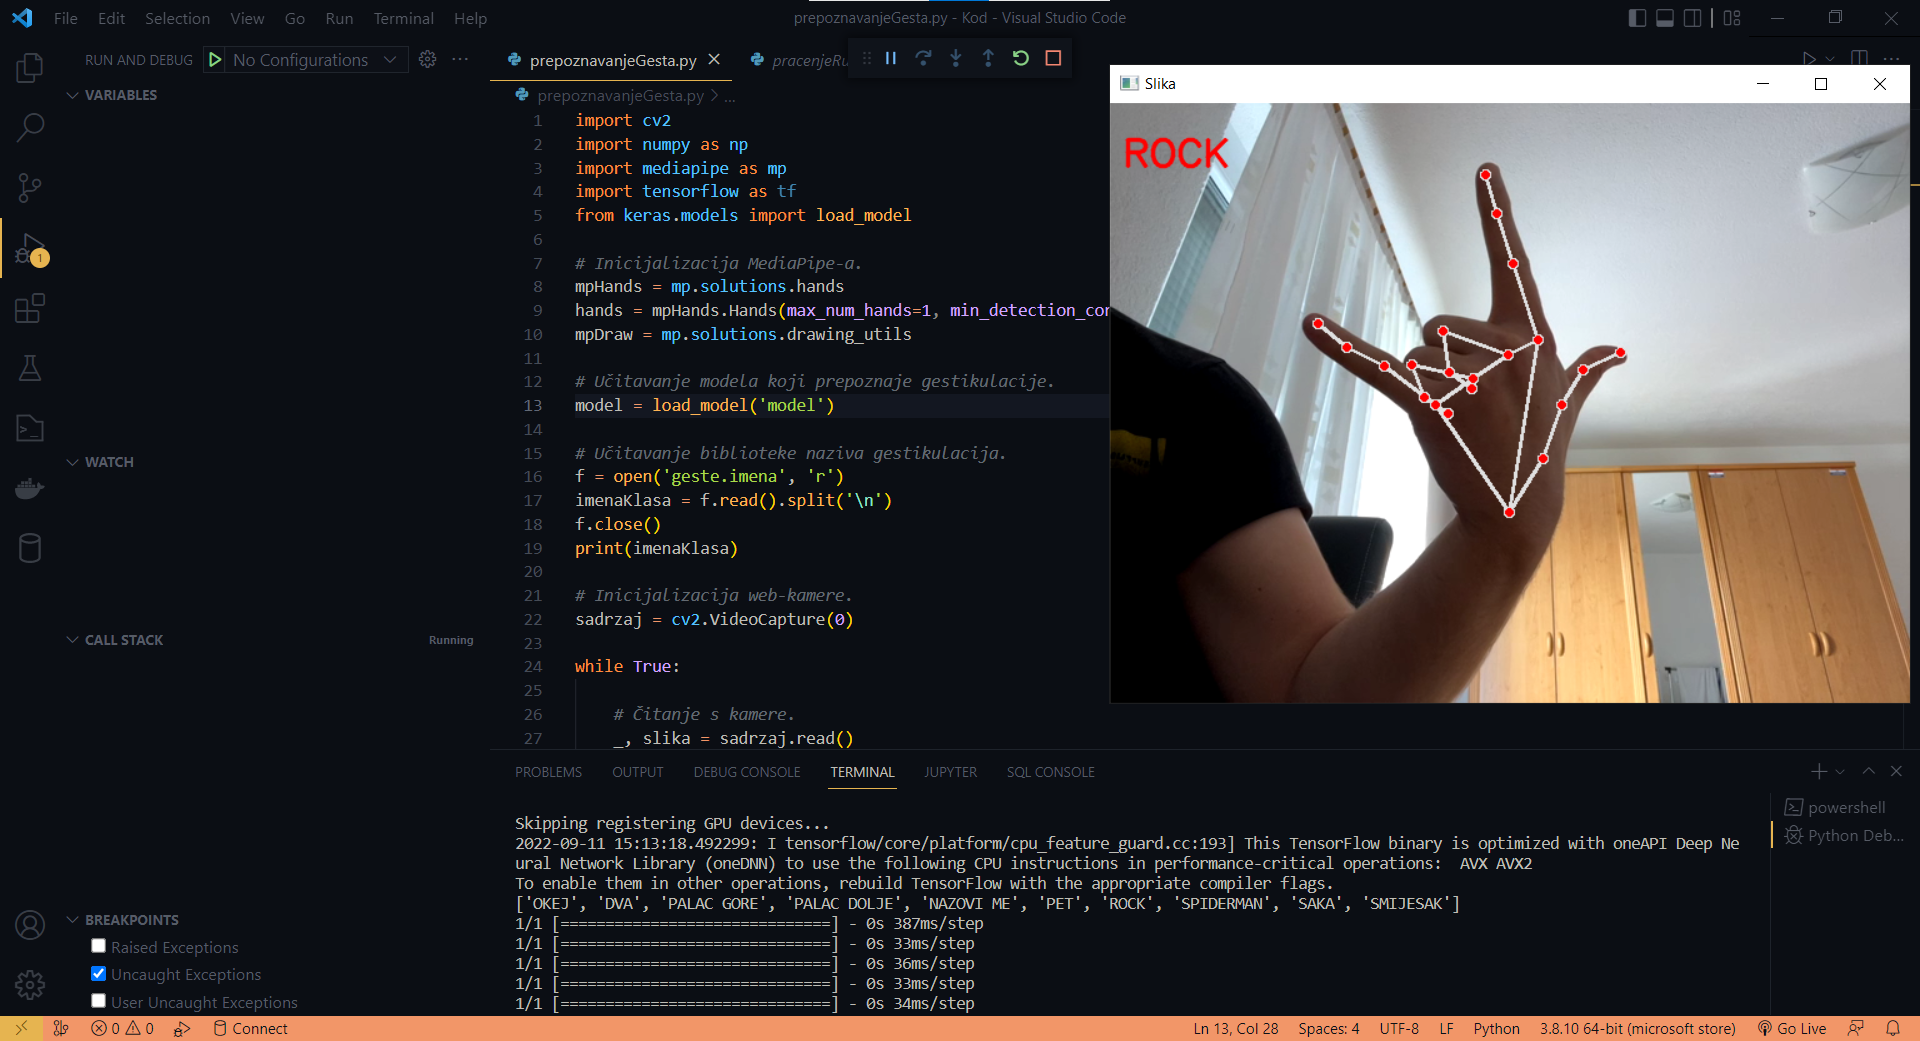
\includegraphics[width=1\textwidth]{slike/rock.png}
    \caption{Prepoznavanje geste}
    \label{fig:rock}
\end{figure}

\chapter{Zaključak}

Računalni vid je popularna tema u radovima o novoj tehnologiji. Drugačiji pristup korištenju podataka je ono što ovu tehnologiju čini drugačijom. Ogromne količine podataka koje se svakodnevno stvaraju, za koje neki ljudi misle da su prokletstvo današnjih generacija, zapravo se koriste za našu dobrobit -- podaci mogu naučiti računala da vide i razumiju objekte. Ova tehnologija također pokazuje važan korak koji naša civilizacija čini prema stvaranju umjetne inteligencije koja može biti sofisticirana poput ljudske.

U radu je prikazano kako u teoriji računalo može prepoznati postoji li određena vrsta objekta na slici, poput prometnog znaka, ljudskog lica, tumora na medicinskoj slici itd. Počevši od samih začetaka ove grane znanosti, obrade slike, razvoja isto tako nove grane umjetne inteligencije dubokog učenja pa sve do primjena njegovih koncepata u računalnom vidu. Primjerice, kada se putem sigurnosnih kamera traži određena osoba, trenutno je moguće suziti izbor na najmanje 10 posto osoba koje kamere detektiraju, što ljudima olakšava posao. I u autonomnoj vožnji samo je pitanje vremena kada će se u potpunosti moći prepustiti vožnja autonomnim vozilima bez ugrožavanja ljudskih života i okoliša.\\
Upravo ta tehnologija (rezolucija kamere, brzina računala), sve je bliža proizvodnji potpuno sigurnih vozila ili prijevoznih sredstava koji ne ugrožavaju živote civila, već samo otklanjaju prijetnje (opasnosti). Daljnji napredak može se postići primjenom kombiniranih tehnologija poput infracrvenih kamera te analizom ljudskih pokreta poput hodanja.\\
Predstavljene su i dvije implementacije, od kojih su kao dio praktičnog dijela rada, jedna implementacija predstavlja detekciju ruke te prikaz njenih gesti u riječi kao rezultat te druga na kojoj se pomoću također gestikulacije ruke, provodi postupak kretnje pokazivača po zaslonu te lijevog klika miša pokazivajući dva podignuta prsta.

Unatoč svom tom nedavnom napretku, koji je bio impresivan, još uvijek se ne nadzire konačno rješenje problema računalnog vida. Međutim, već postoji više zdravstvenih ustanova i poduzeća koja su pronašla načine za primjenu sustava računalnog vida, koje pokreće \textit{CNN}, na probleme u stvarnom svijetu. A ovaj trend vjerojatno neće uskoro prestati.

\makebackmatter
% generira popis korištene literature, popis slika (ako je primjenjivo), popis tablica (ako je primjenjivo) i popis isječaka koda (ako je primjenjivo)

\appendices

\chapter{Programski kôd}

\href{https://github.com/pmatisic/zavrsni}{Poveznica na \textit{GitHub} platformu na kojoj se nalaze programski kôdovi. (Potrebno je kliknuti na ovaj tekst.)}

\end{document}
